%
% UCSD Doctoral Dissertation Template
% -----------------------------------
% Fernando Serrano Paolo <fpaolo@ucsd.edu>
% Version 0 - Jun 1, 2015
%
%
% ----------------------------------------------------------------------
% WARNING: 
%
%   This template has not endorced by OGS or any other official entity.
%   The official formatting guide can be obtained from OGS.
%   It can be found on the web here:
%   http://ogs.ucsd.edu/AcademicAffairs/Documents/Dissertations_Theses_Formatting_Manual.pdf
%
%   No guaranty is made that this LaTeX class conforms to the official UCSD guidelines.
%   Make sure that you check the final document against the Formatting Manual.
%  
%   That being said, this class has been routinely used for successful 
%   publication of doctoral theses.  
%
%   The ucsd.cls class files are only valid for doctoral dissertations.
%
%
% ----------------------------------------------------------------------
% GETTING STARTED:
%
%   Lots of information can be found on the project wiki:
%   http://code.google.com/p/ucsd-thesis/wiki/GettingStarted
%
%
%   To make a pdf from this template use the command:
%     pdflatex template
%
%
%   To get started please read the comments in this template file 
%   and make changes as appropriate.
%
%   If you successfully submit a thesis with this package please let us
%   know.
%
%
% ----------------------------------------------------------------------
% KNOWN ISSUES:
%
%   Currently only the 12pt size conforms to the UCSD requirements.
%   The 10pt and 11pt options make the footnote fonts too small.
%
%
% ----------------------------------------------------------------------
% HELP/CONTACT:
%
%   If you need help try the ucsd-thesis google group:
%   http://groups.google.com/group/ucsd-thesis
%
%
% ----------------------------------------------------------------------
% BUGS:
%
%   Please report all bugs at:
%   http://code.google.com/p/ucsd-thesis/issues/list
%
%
% ----------------------------------------------------------------------
% More control of the formatting of your thesis can be achieved through
% modifications of the included LaTeX class files:
%
%   * ucsd.cls    -- Class file
%   * uct10.clo   -- Configuration files for font sizes 10pt, 11pt, 12pt
%     uct11.clo                            
%     uct12.clo
%
% ----------------------------------------------------------------------



% Setup the documentclass 
% default options: 12pt, oneside, final
%
% fonts: 10pt, 11pt, 12pt -- are valid for UCSD dissertations.
% sides: oneside, twoside -- note that two-sided theses are not accepted 
%                            by OGS.
% mode: draft, final      -- draft mode switches to single spacing, 
%                            removes hyperlinks, and places a black box
%                            at every overfull hbox (check these before
%                            submission).
% chapterheads            -- Include this if you want your chapters to read:
%                              Chapter 1
%                              Title of Chapter
%
%                            instead of
%                              1 Title of Chapter
\documentclass[12pt,chapterheads]{ucsd}



% Include all packages you need here.  
% Some standard options are suggested below.
%
% See the project wiki for information on how to use 
% these packages. Other useful packages are also listed there.
%
%   http://code.google.com/p/ucsd-thesis/wiki/GettingStarted

%% MARGINS
\usepackage[
right=1.3in,
bottom=1in,
]{geometry}


%% MICROTYPE
\usepackage[
activate={true,nocompatibility},
final,
tracking=true,
kerning=true,
spacing=true,
factor=1100,
stretch=10,
shrink=10
]{microtype}
% activate={true,nocompatibility} - activate protrusion and expansion
% final - enable microtype; use "draft" to disable
% tracking=true, kerning=true, spacing=true - activate these techniques
% factor=1100 - add 10% to the protrusion amount (default is 1000)
% stretch=10, shrink=10 - reduce stretchability/shrinkability (default is 20/20)

% CHAPTERS AND SECTIONS
%\usepackage[]{titlesec}
%\titleformat{\chapter}{\normalfont\huge}{\thechapter.}{20pt}{\huge\it}


% FOOTNOTES - formatting the defaul footnotes (reverse indent and marging)
\makeatletter
\renewcommand\@makefntext[1]{\leftskip=2em\hskip-0em\@makefnmark#1} % 2em and -2em
\makeatother

%% AMS PACKAGES - Chances are you will want some or all 
%    of these if writing a dissertation that includes equations.
\usepackage{amsmath, amscd, amssymb, amsthm}
%\usepackage{mathtools}

% Define a command \overbar, which reduces the width of \overline by 1.5mu on each side
\newcommand{\overbar}[1]{\mkern 1.5mu\overline{\mkern-1.5mu#1\mkern-1.5mu}\mkern 1.5mu}

% Define a command \vect, for bold non-italic vector notation
\newcommand{\vect}[1]{\mathbf{#1}} % undergrad algebra version
%\newcommand{\vect}[1]{#1}          % pure math version
%\newcommand{\vect}[1]{\bm{#1}}     % ISO complying version


%% BOLD MATH
\usepackage{bm}

%% SYMBOLS
\usepackage{gensymb}

%% GRAPHICX - This is the standard package for 
%    including graphics for latex/pdflatex.
%    use 'draft' to replace the figures with a black frame
\usepackage[draft]{graphicx}

%% SUBFIG - Use this to place multiple images in a
%    single figure.  Subfig will handle placement and
%    proper captioning (e.g. Figure 1.2(a))
%\usepackage{subfig}

%% CAPTIONS - Use this to customized captions 
\usepackage[font=footnotesize,labelfont=bf]{caption}
\usepackage[leftcaption,raggedright]{sidecap}

%% FONTS - replacements for Computer Modern
% Times
% \usepackage[T1]{fontenc}
% \usepackage{mathptmx}

% Palatino
%\usepackage{mathpazo}

% Bitstream Charter
\usepackage[T1]{fontenc}
\usepackage[charter]{mathdesign} % w/math


% DROP CAPS
\usepackage{lettrine}

%% INDEX
%   Uncomment the following two lines to create an index: 
% \usepackage{makeidx}
% \makeindex
%   You will need to uncomment the \printindex line near the
%   bibliography to display the index.  Use the command
% \index{keyword} 
%   within the text to create an entry in the index for keyword.
%   To compile a LaTeX document with an index the 'makeindex'
%   command will need to be run.  See the wiki for more details.

% BIBLIOGRAPHY - Set to be handled with LaTeX + BibLaTeX
\usepackage[
backend=bibtex,
style=alphabetic,
citestyle=authoryear,
firstinits=true,
isbn=false,
url=false,
doi=true,
eprint=false,
refsegment=chapter,    % if using a global .bib file
%refsection=chapter,   % if using multiple .bib files
]{biblatex}

\bibliography{myrefs}  % global bibliography file

%% HYPERLINKS
%   To create a PDF with hyperlinks, you need to include the hyperref package.
%   THIS HAS TO BE THE LAST PACKAGE INCLUDED!
%   Note that the options plainpages=false and pdfpagelabels exist
%   to fix indexing associated with having both (ii) and (2) as pages.
%   Also, all links must be black according to OGS.
%   See: http://www.tex.ac.uk/cgi-bin/texfaq2html?label=hyperdupdest
%   Note: This may not work correctly with all DVI viewers (i.e. Yap breaks).
%   NOTE: hyperref will NOT work in draft mode, as noted above.
% \usepackage[colorlinks=true, pdfstartview=FitV, 
%             linkcolor=black, citecolor=black, 
%             urlcolor=black, plainpages=false,
%             pdfpagelabels]{hyperref}
% \hypersetup{ pdfauthor = {Your Name Here}, 
%              pdftitle = {The Title of The Dissertation}, 
%              pdfkeywords = {Keywords for Searching}, 
%              pdfcreator = {pdfLaTeX with hyperref package}, 
%              pdfproducer = {pdfLaTeX} }


\begin{document}



%% FRONT MATTER
%
%  This includes the title, degree, dedication, vita, abstract, etc..
%%
% Front pages
% -----------
% Jun 1, 2015 
%
%


%% REQUIRED FIELDS -- Replace with the values appropriate to you

% No symbols, formulas, superscripts, or Greek letters are allowed
% in your title.
\title{Interannual and decadal variations of Antarctic ice shelves using
multi-mission satellite radar altimetry, and links with oceanic and atmospheric
forcings}

\author{Fernando Serrano Paolo}
\degreeyear{2015}

% Master's Degree theses will NOT be formatted properly with this file.
\degreetitle{Doctor of Philosophy} 

\field{Earth Sciences}

\chair{Professor Helen A. Fricker}
% Uncomment the next line iff you have a Co-Chair
% \cochair{Professor Cochair Semimaster} 
%
% Or, uncomment the next line iff you have two equal Co-Chairs.
%\cochairs{Professor Chair Masterish}{Professor Chair Masterish}

%  The rest of the committee members  must be alphabetized by last name.
\othermembers{
Professor Sarah T. Gille\\
Professor Jean-Bernard Minster\\
Professor Larie Padman\\ 
Professor David T. Sandwell\\
Professor Falko Kuester\\
}
\numberofmembers{6} % |chair| + |cochair| + |othermembers|


%% START THE FRONTMATTER
%
\begin{frontmatter}

%% TITLE PAGES
%
%  This command generates the title, copyright, and signature pages.
%
\makefrontmatter 

%% DEDICATION
%
%  You have three choices here:
%    1. Use the ``dedication'' environment. 
%       Put in the text you want, and everything will be formated for 
%       you. You'll get a perfectly respectable dedication page.
%   
%    2. Use the ``mydedication'' environment.  If you don't like the
%       formatting of option 1, use this environment and format things
%       however you wish.
%
%    3. If you don't want a dedication, it's not required.
%
%
\begin{dedication} 
  To two, the loneliest number since the number one.
\end{dedication}


% \begin{mydedication} % You are responsible for formatting here.
%   \vspace{1in}
%   \begin{flushleft}
% 	To me.
%   \end{flushleft}
%   
%   \vspace{2in}
%   \begin{center}
% 	And you.
%   \end{center}
% 
%   \vspace{2in}
%   \begin{flushright}
% 	Which equals us.
%   \end{flushright}
% \end{mydedication}



%% EPIGRAPH
%
%  The same choices that applied to the dedication apply here.
%
\begin{epigraph} % The style file will position the text for you.
\emph{
It should never assert as argument the authority of any man, by excellent and illustrious that is... It is extremely unfair to fold one's own feeling to a slavish reverence towards others; being submissive is worthy of mercenaries or slaves and contrary to the dignity of human freedom; it is utmost stupidity to believe by inveterate custom; it is irrational thing to conform with an opinion because of the number of those who have it. We must instead always seek a real and necessary reason... \\
and listen to the voice of nature.
} \\
---Giordano Bruno \\
(burned at the stake, 1548--1600)
\end{epigraph}

% \begin{myepigraph} % You position the text yourself.
%   \vfil
%   \begin{center}
%     {\bf Think! It ain't illegal yet.}
% 
% 	\emph{---George Clinton}
%   \end{center}
% \end{myepigraph}


%% SETUP THE TABLE OF CONTENTS
%
\tableofcontents
\listoffigures  % Uncomment if you have any figures
\listoftables   % Uncomment if you have any tables



%% ACKNOWLEDGEMENTS
%
%  While technically optional, you probably have someone to thank.
%  Also, a paragraph acknowledging all coauthors and publishers (if
%  you have any) is required in the acknowledgements page and as the
%  last paragraph of text at the end of each respective chapter. See
%  the OGS Formatting Manual for more information.
%
\begin{acknowledgements} 
 Thanks to whoever deserves credit for Blacks Beach, Porters Pub, and
 every coffee shop in San Diego. 

Chapter 2, in full, has been submitted for publication of the material
as it may appear in {\it Remote Sensing of Environment} 2015.
Paolo, Fernando. S.; Fricker, Helen A.; Padman, Laurie.
The dissertation author was the primary investigator and author of this paper.

Chapter 3, in full, is a reprint of the material as it appears
in {\it Science} 2015.
Paolo, Fernando. S.; Fricker, Helen A.; Padman, Laurie.
The dissertation author was the primary investigator and author of this paper.

Chapter 4, in part [or in full?], is currently being prepared for submission
for publication of the material.
Paolo, Fernando. S.; Fricker, Helen A.; Padman, Laurie.
The dissertation author was the primary investigator and author of this material.

 
\end{acknowledgements}


%% VITA
%
%  A brief vita is required in a doctoral thesis. See the OGS
%  Formatting Manual for more information.
%
\begin{vitapage}
\begin{vita}
  \item[2007] B.~S. in Oceanography, University of S\~ao Paulo, Brazil
  \item[2009] M.~S. in Geophysics, University of S\~ao Paulo, Brazil
  \item[2015] Ph.~D. in Geophysics, University of California, San Diego 
\end{vita}
\begin{publications}
  \item Your Name, ``A Simple Proof Of The Riemann Hypothesis'', \emph{Annals of Math}, 314, 2007.
  \item Your Name, Euclid, ``There Are Lots Of Prime Numbers'', \emph{Journal of Primes}, 1, 300 B.C.
\end{publications}
\end{vitapage}


%% ABSTRACT
%
%  Doctoral dissertation abstracts should not exceed 350 words. 
%   The abstract may continue to a second page if necessary.
%
\begin{abstract}
  This dissertation will be abstract. 
\end{abstract}


\end{frontmatter}






%% DISSERTATION

% A common strategy here is to include files for each of the chapters. I.e.,
% Place the chapters is separate files: 
%   chapter1.tex, chapter2.tex
% Then use the commands:


% Chapter 1 - Introduction 
% ------------------------
% Jun 6, 2015


\chapter{Introduction and background}

\section*{Ice shelves, ice-sheet and sea-level rise}

\lettrine[lines=2]{T}{he Antarctic Ice Sheet loses} most of its mass from its fringing ice shelves\footnote{
The ice shelves loose their mass through either iceberg calving or basal melting
(see Figure \ref{ch1fig1}).},
the marginal floating extensions of inland glaciers and ice streams. More than 80\% of
Antarctica's ice drains through the ice shelves, where most of the mass
lost from the ice sheet is transferred to the ocean. The Antarctic Ice Sheet
contains ice equivalent to $\sim$58 m of global sea-level rise
\parencite{Fretwell2013}, and has been losing mass at an average rate of
$\sim$71 Gt year$^{-1}$ (gigatonnes per year) between 1992 and 2011
\parencite{Shepherd2012}\footnote{This is equivalent to a contribution of
(slightly over) 6\% to the total sea-level rise of $\sim$3.2 mm year$^{-1}$
(CITE).}. A moderate loss of 2\% of the Antarctic Ice Sheet is sufficient to rise
the global sea level by $\sim$1 m. More important, however, is the accelerated
state of this ice-loss rate, as has been observed during the past decade
\parencite{Shepherd2012, Sutterley2014, Velicogna2009, Chen2009, Harig2015}, 
which raises significant concern on future ice-sheet behaviour and its
contribution to global sea level. 

Located at the boundary between the ice sheet, atmosphere and ocean,
Antarctica's ice shelves are potentially vulnerable to changes in both
atmospheric and oceanic conditions (Figure \ref{ch1fig1}), making them sensitive indicators of
large-scale climate change. For more than two decades, rapid
changes have been occurring in the extent and thickness of many Antarctic ice
shelves, particularly along the Antarctic Peninsula and the Amundsen Sea
sector of West Antarctica \parencite{Cook2010, Pritchard2012, Shepherd2010,
Wingham2009, Zwally2005, Fricker2012}(Figure \ref{ch1fig2}[some figure
showing ice-shelf loss?]). It is, therefore, through the ice shelves that variations in
oceanic and atmospheric states force changes in the grounded ice sheet.

In the past decade, considerable progress has been made in understanding the
fundamental role that the ice shelves play in restraining the grounded ice sheet
flow [Schoof; Goldberg; Hilmar; etc.]. Ice shelves exert a back-stress on
grounded tributary-glaciers and ice streams resulting from drag forces
at the ice-bedrock interface. This resistive stress, known as \emph{buttressing effect},
holds back the ice flow from the ice-sheet interior to the ocean.
With loss of back-stress due to ice-shelf shrinkage or breakup, ice discharge
increases scaling nonlinearly with grounding line (GL)\footnote{The ground line
is the dynamic boundary between the grounded ice sheet and the floating ice shelves;
where glaciers detach from the bedrock and start afloat.} thickness to
compensate for the reduction in \emph{buttressing} [7, 21]. This nonlinear dynamics,
flow $\propto$ thickness$^{n \geqslant 3}_\text{GL}$, becomes particularly important in
regions where (a) the ice sheet is
grounded below sea level (marine ice sheet) and (b) the bed deepens inwards
(retrograde bed slope). Such configuration gives rise to a condition of unstable
equilibrium known as \emph{marine ice-sheet instability} (Figure \ref{ch1fig3}),
first proposed in the 70s by [see Hilmar for the right citations].

There have been recent rapid advances in identifying the dynamical processes by which the
ocean can control ice-sheet mass loss and associated sea-level rise. Studies have shown that
increased ocean-forced basal melting of ice shelves, accelerating flow in adjacent grounded ice,
is responsible for the majority of current Antarctic ice sheet loss \parencite{Rignot2008,
Pritchard2009}. Dramatic grounding line retreat as a consequence
of intensified basal melting has induced extensive land ice thinning \parencite{Wingham2009,
Pritchard2009, Rignot2014}, and faster flow rates have followed ice shelf collapses
due to the reduction in \emph{buttressing} \parencite{Rignot2004, Rignot2005, Scambos2004}.
Indeed, 87\% of all Antarctic Peninsula (AP) tidewater glaciers are known to be retreating
\parencite{Cook2005}, and dynamic thinning (increase strain rates due to flow acceleration)
has occurred around the AP \parencite{Rignot2008, Pritchard2009}.
These observations have been interpreted as evidence that
ocean forcing can lead to rapid changes in ice sheet dynamic flow and its subsequent
contribution to sea-level rise. Despite this progress, our understanding of these processes
is still too rudimentary to allow prediction of ice sheet change under projected
future climate states.

In essence, because the grounded ice sheet changes in response to perturbations in the ice
shelves, understanding variations in the state of the ice shelves is key to
identify relationships between observed ice loss and large-scale climate variability.
There are two complementary ways forward: to develop our understanding of the actual mass
loss processes, so they can be better represented in models; and to empirically relate observed
ice-sheet change to ocean and atmospheric variability. This dissertation focuses on the second
approach.

\section*{Satellite altimetry and change detection}

Continuous observations of ice shelves over long time periods are required to determine stability,
monitor change, and identify general relationships between observed changes and ocean
variability. Given the vast size of Antarctica, its remote location and challenging field conditions,
space-based techniques are the only practical way to monitor the ice sheet.
Much of our current understanding of how ice-shelf processes couple ice-sheet changes to climate variability comes from analyses of trends in surface elevation change, $\partial h / \partial t$, derived from satellite radar and laser altimeter data \parencite{Zwally2005, Shepherd2010, Pritchard2012, Fricker2012}.
In particular, satellite radar altimeters\footnote{Radar antennas mounted on satellites flying at
$\sim$780 km of altitude.}
have provided the longest set of continuous observations over the Antarctic and Greenland ice sheets, and have revolutionized the way we study these ice masses. Maps of ice-shelf height change at high spatial resolution have also been developed using measurements from a satellite laser altimeter (ICESat\footnote{Something about ICESat.}) \parencite{Pritchard2012}, but the time span of this data set only covered the period 2003--2008 (5 years). In contrast, satellite radar altimeters (RA) have been providing
measurements of the ice shelves since 1978\footnote{Although another radar altimeter flew before
this date over the ice sheets (the GEOS-3), its experimental measurements were not
useful for ice-sheet change determination.} \parencite{Zwally1983, Zwally1989, Davis1998, Martin1983}. However,
historical RA missions like Seasat (1978) and Geosat (1985--1989) were limited to orbit latitudes north of 72\degree S (south of 72\degree N for Greenland) and, although insufficient for whole ice sheet studies, this coverage did capture a large portion of the fringing ice shelves and marginal grounded ice.

A satellite radar altimeter measures the satellite-to-surface round-trip travel time of the emitted electromagnetic waves\footnote{The standard altimeters used in this study operated in the Ku-band (microwaves): $f =$ 12--18 GHz, $\lambda =$ 2.5--1.7 cm} and their phase shift (Figure \ref{ch1figX}). As electromagnetic waves travel through the atmosphere, they can be delayed by water vapour or by ionization. Once these effects are corrected for, the final range $R$ is estimated with high precision\footnote{The strength of satellite radar altimeters is their single-measurement high precision, which is fundamental for estimating changes (more so than accuracy).}. The radar-altimeter functional response over ice surfaces is considerably more complex than over the oceans. Causal factors identified in the complex backscatter response over ice sheets include sloping surfaces, surface undulations with characteristic wavelengths on the same spatial scale as the altimeter beam-limited footprint, off-track reflections, dynamic lag of the altimeter tracking circuit (on-board, which requires an off-board post-processing \emph{retracking} step), and spatio-temporal variations in the ice-surface properties. \parencite{Martin1983}. \emph{Retracking} methods using the altimeter return pulse waveforms (Figure \ref{ch1figX}) give range corrections that are typically several meters, and significant differences are found between different \emph{retracking} algorithms \parencite{Davis1996}. We then have the ellipsoidal height estimated by an altimeter as

\begin{equation}
  h = h_\text{s} - R - \epsilon
\end{equation}

where $h$ is the height of the surface with respect to the ellipsoid, $h_\text{s}$ is the satellite's altitude, $R$ is the satellite-to-surface measured range, and $\epsilon$ represents the atmospheric path delay (accounted for). By performing repeated measurements one can track changes in the ice-shelf height, that relates to the ice-shelf mass balance as follows

\begin{equation}
\begin{split}
  \frac{\partial h}{\partial t} &= \frac{\partial \Delta}{\partial t}
    - M \, \frac{\partial}{\partial t} \, \rho^{-1}_\text{w}
    + \int^M_0 \text{d}m \, \frac{\partial}{\partial t} \, \rho^{-1}_\text{f}(m) \\
    &\quad + ( \rho^{-1}_\text{i} - \rho^{-1}_\text{w} ) 
              \left( \dot{M}_\text{s} + \dot{M}_\text{b} + \vect{u} \cdot \nabla M
              + M \nabla \cdot \vect{u} \right)
\end{split}
\end{equation}

where...[explanation of each component]

With the demonstrated capability of all-wheather-operational radar altimeters
(Figure: RA measurement scheme)
a new era of polar science was set. More than two decades of modern (global) RA missions,
including the ERS-1 (1992--1996), the ERS-2 (1995--2003), the Envisat (2002--2012), and
the Cryosat-2 (2010--present), have improved dramatically our understanding of ice-sheet
dynamics and its relation to measured sea-level rise [CITE?]. In general, however,
studies focusing on the ice shelves using RA have under-exploited these data,
reporting linear height-trends for a fraction---and usually for broad regions---of the complete (modern-era) RA data set \parencite{Shepherd2003, Shepherd2010, Zwally2005}.

In addition, satellite observations over the past two decades have provided estimates of
the Antarctic mass budget, which vary widely according the method they are based upon---from
$+$50 to $-$250 Gt year$^{-1}$ for 1992--2009 \parencite{Zwally2011}. As reported in
\textcite{Zwally2011}:

\begin{quotation}
\noindent
Generally, the range of estimates in IPCC07\footnote{Define IPCC07.} encompassed the errors listed in the studies, but as noted in the report, a mid-range value does not indicate a more reliable estimate, and the composite errors listed in each study do not define confidence limits because important components lack formal statistical derivation. This caution on the error estimates applies to all studies regardless of methods of data collection and analyses.
\end{quotation}

This highlights the need to account for uncertainties in a more consistent way, as well as analyzing these inherently noisy and complex measurements with robust statistical estimation procedures.

\section*{Scientific objectives}

[SEE "ORGANIZATION" EXAMPLE OF BOOK: TREES, MAPS, AND...]

This PhD thesis seeks to address the following scientific questions:

\begin{enumerate}
  \item[a)] Has $\partial h / \partial t$ for Antarctic ice shelves been constant
  or has it varied over time?
  \item[b)] Are the observed changes restricted to particular regions or do they
  occur in a larger scale?
  \item[c)] What are the spatial patterns of coherence in $\partial h / \partial t$
  around Antarctica?
  \item[d)] Are there links between interannual variability of the ice shelves and
  oceanic and atmospheric variability?
\end{enumerate}

To be achieved with the conclusion of the following objectives:

\begin{enumerate}
  \item[i)] {\it Derive reliable time series of elevation change} ({\sc Chapter 2}). Improve and
  extend the procedures for extracting height changes from multi-mission RA
  records, deriving reliable long-term, continuous time series in a
  high-resolution grid for consistent trend analysis
  \item[ii)] {\it Quantify long-term trends} ({\sc Chapter 3}). Analyze long-term changes for
  all Antarctic ice shelves spanning a time period of nearly two decades,
  mapping in time and space the height-/volume-change rates, acceleration
  and associated uncertainties.
  \item[iii)] {\it Analyze interannual-to-decadal variability} ({\sc Chapter 4}). Use the
  extended time series and spatial maps to seek relationships between
  ice-shelf-height fluctuations and known modes of variability in the
  atmosphere and the ocean ({\it e.g.}, El Ni\~{n}o Southern Oscillation).
\end{enumerate}

\section*{Thesis outline}

This thesis is organized in four chapters. Each chapter was designed as a self-contained piece of work to address the general objectives proposed in this dissertation (above). {\sc Chapter~1} (this current chapter) presents an introduction to the scientific questions being addressed and the background necessary to follow the work done in Chapters 2--4. {\sc Chapter~2} describes the full methodology implemented in this study (partially developed and partially modified from previous works) to construct the longest, continuous, high-resolution (in time and space) time series of changes in ice-shelf surface-height from multiple satellite radar altimeters. In this chapter the RA data and corrections are discussed, and new processing approaches are proposed. This chapter is currently in review for publication in the journal {\it Remote Sensing of Environment}. {\sc Chapter~3} describes the trend analysis approach implemented in the ice-shelf-height time-series product (derived in Chapter 2), as well as reports and discusses the findings, which have advanced significantly our understanding on the state of the Antarctic ice shelves. This chapter is published in the journal {\it Science}. {\sc Chapter~4} focuses on the variability analysis of the ice-shelf-height time series. This chapter investigates the origin of interannual fluctuations in the ice-shelf volume, and seeks to understand the links between observe changes and large-scale climate variability. This chapter is currently in preparation for submission \emph{after} the dissertation defense.

\section*{Summary of results}

This thesis presents a method for optimal analyses of ice-shelf-height data from multiple satellite RAs and estimation of uncertainties in the resulting data products. We constructed an 18-year time series of height changes at $\sim$30 km grid cells and $\sim$3 month intervals over Antarctica's floating ice shelves. Our data set allowed us to estimate, with high statistical confidence (95\% level), the temporal progression and spatial structure of ice-shelf height changes in Antarctica between 1994 and 2012.

We have demonstrated that: Substantial averaging both in time and space is required to construct RA height records over floating ice shelves. Densification of the surface greatly affects the height-change estimate, and backscatter correction significantly reduces this effect. Densification is a more important effect than penetration in biasing the height-change estimates over the ice shelves. Given the high interannual-to-decadal variability that is present, a simple straight-line fit fails to capture the underlying trends, some degree of curvature in the trend is needed. Polynomial trends allow to obtain information on the evolution and spatial structure of changes, such as instantaneous rate of change (derivative of the trend) and average acceleration (slope of the derivative). Given the convoluted nature of the error sources, we propose that a top-down approach for uncertainty estimation (e.g., bootstrap applied to time-dependent data) constitutes a more accurate alternative for error analysis.

We have shown that Antarctic ice-shelf volume
loss is accelerating. In the Amundsen Sea,
some ice shelves buttressing regions of grounded
ice that are prone to instability have experienced
sustained rapid thinning for almost two decades.
If the present climate forcing is sustained, we
expect a drastic reduction in volume of the rapidly
thinning ice shelves at decadal to century
time scales, resulting in grounding-line retreat
and potential ice-shelf collapse. Both of these processes
further accelerate the loss of buttressing,
with consequent increase of grounded-ice
discharge and sea-level rise. On smaller scales,
ice-shelf thickness variability is complex, demonstrating
that results from single satellite missions
with typical durations of a few years are
insufficient to draw conclusions about the long-term
response of ice shelves. Large changes occur
over a wide range of time scales, with rapid variations
of ice-shelf thickness suggesting that ice
shelves can respond quickly to changes in oceanic
and atmospheric conditions.

\section*{Future research}

Our preliminary results on the variability analysis performed to the 18-year record of ice-shelf height changes, show that there is significant interannual fluctuations in Antarctic ice-shelf volume. Besides advancing our understanding on how the oceanic and atmospheric forcing impacts the ice sheet, this has also important implications for estimating changes in freshwater fluxes around Antarctica. With the aid of innovative mathematical tools for analyzing sets of short and noisy records (e.g., multi-variate singular spectrum analysis), we have estimated the spectrum of sub-decadal changes for some key regions in West Antarctica. We found statistically significant peaks (energy content) in two particular frequency bands: $\sim$1 year (the expected contribution from the seasonal cycle) and $\sim$4--6 years. Interestingly, the latter coincides with the characteristic spectral signature of El Ni\~no Southern Oscillation (ENSO) as derived from the Sourthern Oscillation Index (SOI). The ENSO has been shown to affect sea-surface pressure and, consequently, sea-ice conditions in the Amundsen and Bellingshausen seas. Although the Antarctic response to ENSO forcing is not ubiquitous, it is reasonable to expect that this large-scale climate variation will be felt by the floating ice shelves as well. Investigating potential linkages between tropical-climate variability and changes in the Antarctic ice shelves is the subject of a planned postdoctoral project.

[MAKE REFERENCES SINGLE-SPACED WITH A DOUBLE SPACE BETWEEN ENTRIES]
\printbibliography[segment=1,heading=subbibliography]

%
% Chapter 2 - Method
% ------------------
% Jul 1, 2015
%

\chapter{Developing optimal decadal records of Antarctic ice-shelf height change from multiple satellite radar altimeters}


\section*{}
\noindent
Antarctica's ice shelves, the floating extensions of the ice sheet, exert an important dynamic constraint on the flow of ice from the grounded ice sheet to the ocean, and hence on changes in global sea level. Thinning of an ice shelf reduces its ability to restrain the ice discharge from the grounded ice-sheet interior. However, our understanding of how ice-shelf processes couple ice-sheet changes to climate variability is still rudimentary. In part, this is due to the brevity and low resolution of surveys of ice-shelf thickness relative to the time scales on which ice-sheet mass fluctuates. We present optimal procedures to construct 18-year (1994--2012) time series of ice-shelf surface height around the entire Antarctic continent by merging data from multiple overlapping satellite radar altimeter missions (ERS-1, ERS-2, and Envisat). We apply an averaging scheme to enhance the signal-to-noise ratio of height changes over the floating ice shelves, and extract low-order polynomial trends using a robust approach accounting for both bias and variance in the fit (regularized regression with cross-validation). We identify the main processes affecting the estimation of ice-shelf height from satellite radar altimeters. We estimate uncertainties by bootstrap resampling of the residuals of the fit, allowing us to construct formal confidence intervals (unlike the standard error-propagation approach). Our results show that, for the ice shelves, densification of the surface is a more important effect than penetration of the radar signal in biasing the estimated height changes. The 18-year record of surface height allows us to map the temporal progression and spatial structure of changes in ice-shelf height, which provides insights on how ice shelves respond to the changing atmospheric and oceanic conditions.

\section{Introduction}

The Antarctic Ice Sheet contains ice above floatation equivalent to ~58 m of global sea-level rise \parencite{Fretwell2013} and, over centennial-to-millennial time scales, plays an important role in pacing sea-level changes \parencite{Alley2005}. Satellite measurements over the past two decades show mass loss from the grounded ice sheet \parencite{Shepherd2012} including accelerating loss in the Amundsen Sea Embayment \parencite{Sutterley2014}, a region with large potential for sea level rise contribution \parencite{Rignot2014, Joughin2014}. There is an urgent need to understand the mechanisms behind these current changes as a step towards predicting Antarctica's contribution to global sea-level change over the next century. 

Most ice mass loss from Antarctica takes place through iceberg calving and basal melting from the ice shelves, the floating extensions of the ice sheet \parencite{Depoorter2013, Joughin2012, Rignot2013}. Ice shelves restrain the discharge of grounded ice into the ocean through a buttressing effect \parencite{Joughin2011, Schoof2007}. Small perturbations in the adjacent oceanic and atmospheric conditions can have a large impact on the extent and thickness of ice shelves \parencite{Dutrieux2014, Rignot2004, Scambos2004}, which reduces their buttressing capability. The response of ice shelves to climate changes is, therefore, a key component in assessing future loss of grounded ice.

Our understanding of the many processes that affect ice-shelf mass balance is too rudimentary to allow prediction of ice-sheet change under projected future climate states. There are two complementary ways forward: to develop our theoretical framework of the actual mass-loss processes so they can be better represented in models; and to empirically relate observed ice-sheet change to ocean and atmospheric variability. In a recent study \parencite{Paolo2015} we reported changes in Antarctic ice shelf height, and inferred thickness during the 18-year period 1994--2012. The temporal and spatial resolutions of that record were ~3 months and ~30 km, respectively. This record will be used to improve knowledge of ice-shelf response to climate by comparing measured variability of ice thickness with measured or modeled changes in the ocean and atmosphere. This continuous, highly-resolved record overcomes the limitations of previous studies of ice-shelf thickness, which analyzed much shorter records and/or predominantly reported simple linear trends for large areas \parencite{Pritchard2012, Shepherd2010, Zwally2005}.

In this paper we document comprehensive methods for constructing continuous records from multiple satellite radar altimeters to obtain reliable time series of height change over the longest possible time period, providing detailed justification for the data processing approach used by \textcite{Paolo2015}. We present optimal procedures for merging data from three overlapping satellite missions, enhancing the signal-to-noise ratio of changes in ice-shelf height, and extracting 18-year mean trends and acceleration. We introduce an alternative approach to the standard error propagation for the uncertainty analysis: bootstrapping applied to time-dependent data. The method reveals complex patterns of ice-shelf height variability in both time and space.

\section{Satellite radar altimeter missions}
\label{sat-ra}

We used data from three European Space Agency (ESA) satellite radar altimeter (RA) missions: the European Remote Sensing Satellite-1 and Satellite-2 (ERS-1, 1991--1996; and ERS-2, 1995--2003); and the Environmental Satellite (Envisat, 2002--2012). Each satellite carried a standard pulse-limited altimeter with a footprint size of $\sim$3--5 km over the ice sheets. For reasons explained in Section \ref{sat-ra}, below, we do not use the first two years of ERS-1 data, resulting in an 18-year continuous record for 1994--2012.

ERS-1 was launched on July 1991 and operated between December 1991 and June 1996. It flew at an altitude of $\sim$785 km with an inclination of 98.5 degrees (latitudinal limit of 81.5$^\circ$), with three different orbital repeat periods: 3-day (Ice Phase, December 1991 to March 1992 and December 1993 to April 1993), 35-day (Multidisciplinary Phase, April 1992 to December 1993 and March 1995 to June 1996) and 168-day (Geodetic Phase, April 1994 to March 1995). ERS-2 was launched on April 1995 and operated from May 1995 to June 2003 in an orbit with a repeat period of 35 days, exactly following the ERS-1 35-day orbit. In June 2003 the on-board tape recorder used for the RA data failed, and the mission continued without altimetry until July 2011. The RA system on these two satellites was based on a linearly polarized antenna at 13.8 GHz Ku-band, yielding along-track measurements (several radar echoes averaged) that are $\sim$340 m apart (sampling rate of 20 Hz).

The ERS-1/ERS-2 orbit covered about 85\% of the Antarctic ice-shelf area, missing only the southern portions of the large Filchner-Ronne (Figure \ref{c2f1}) and Ross ice shelves. Over the ice shelves, ERS-1 and ERS-2 operated in both a standard 'ocean mode' and a specialized 'ice mode', alternating between them. The range window (the segment of return echo that is recorded) for ice mode was four times wider than for ocean mode, increasing the chances of capturing return signals over rough topographic surfaces. However the broader range window resulted in four times coarser sampling of the return waveform, leading to a less precise estimation of arrival time and, therefore, of the surface height.

Envisat was launched in March 2002 into the same 35-day orbit as ERS-1 and ERS-2, providing data at the same 20 Hz sampling rate. The altimeter on this satellite (RA-2) \parencite{Roca2009}, a linearly-polarized radar, operated via a single antenna dish on the Ku-band (13.6 GHz) and S-band (3.2 GHz). This dual frequency enables the correction of height-measurement errors introduced by the ionosphere. RA-2 had an improved precision over ice surfaces compared to the ERS altimeters, and operated with three sampling modes: 'fine', 'medium' and 'coarse', which differ by their sampling of the return waveform. Envisat stopped operating in April 2012.

We obtained Level-2 RA data as Ice Data Records (IDR) for each mission from the NASA/GSFC's Ice Altimetry group ({\tt http://icesat4.gsfc.nasa.gov/}). At GSFC, the RA waveforms were retracked using a multi-parameter range-retracking algorithm (the $\beta$-retracker) \parencite{Martin1983}. The following corrections were applied by GSFC: atmospheric range corrections; instrument corrections; slope corrections; ocean and solid earth tides \parencite{Brenner1983, Zwally2001, Zwally2005}; (for ERS) removal of a 40.9 cm bias from ERS-1 heights to account for a change in instrument parameter used for ERS-2 \parencite{Femenias1996}; corrections for drifts in the ultra-stable oscillator and bias changes in the scanning point target response that are obtained from ESA; and upgraded orbits (DGM-E04 orbits for ERS) which have a radial orbit precision of 5-6 cm \parencite{Scharroo1998}.


\begin{figure}[!ht]
  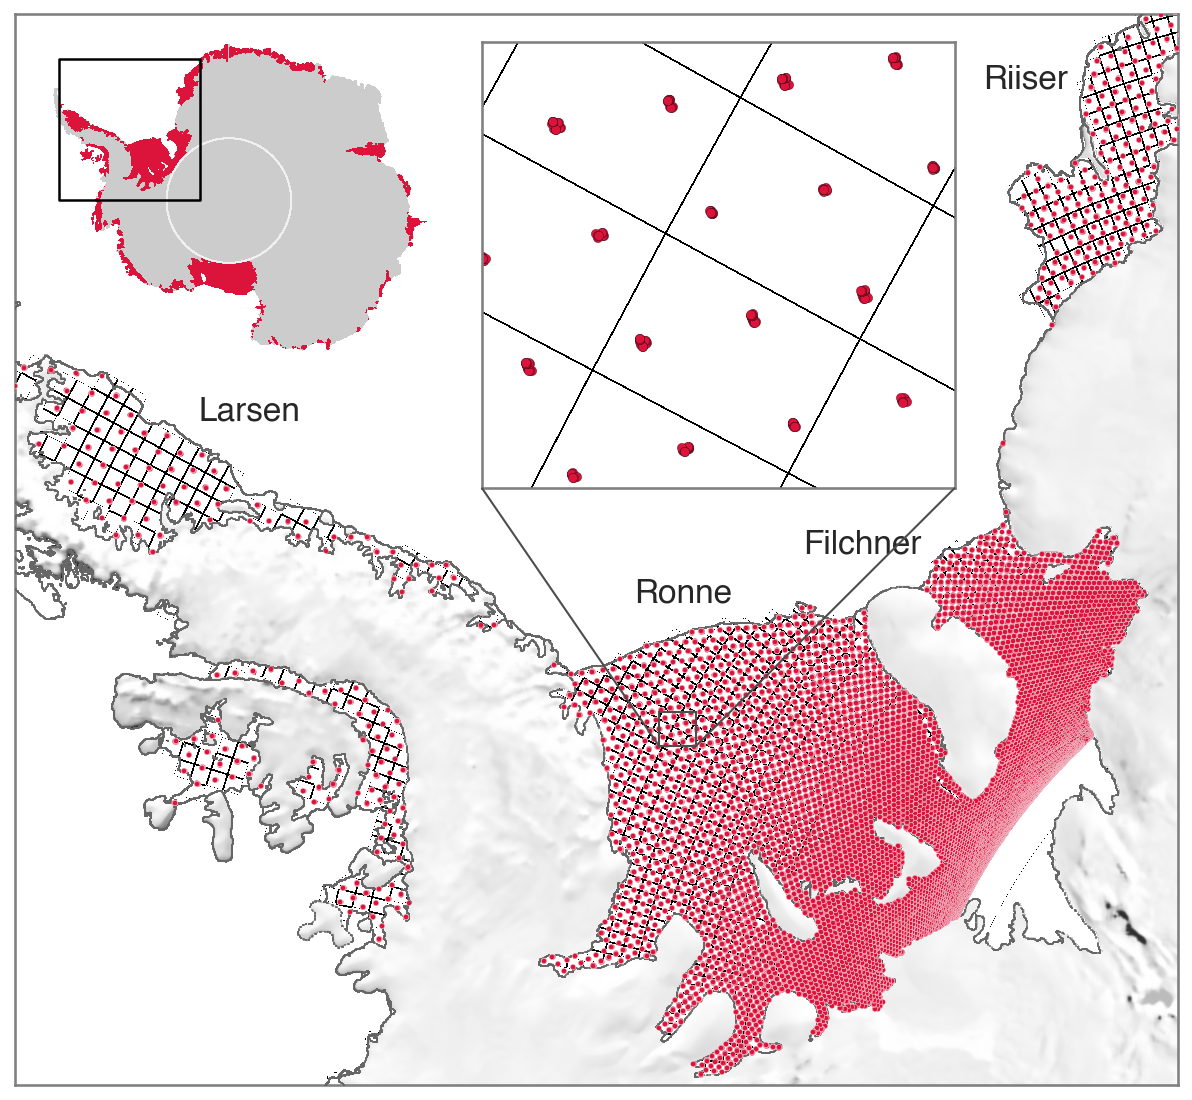
\includegraphics[width=\textwidth]{../img/map_xovers_grid_v8.png}
  \caption{ERS-1 radar altimeter data coverage over the Weddell Sea region of Antarctica for a typical 3-month period with the 35-day repeat orbit. Red dots are crossover locations on the ice shelves. The $\sim$30-km grid that we used to average the crossovers is overlaid. 
  ice shelves.} 
  \label{c2f1}
\end{figure}


\section{Processing satellite radar altimeter data}

Our determination of height changes over the ice shelves from multi-mission satellite RA data is based on crossover analysis [E.G.,]\parencite[e.g.,][]{Davis2004, Wingham2009, Zwally2005}, which estimates change in surface height at intersections between time-separated ascending and descending satellite tracks. Along-track analysis methods that provide higher point density have recently been introduced \parencite{Flament2012, Moholdt2010, Pritchard2012}; however, crossover analysis remains the most precise technique since differences are derived from precisely co-located height estimates on the ascending and descending tracks. The spacing of crossovers becomes much smaller as latitude approaches the satellite's turning point (Figure \ref{c2f1}).

In this section we describe the steps required to process RA data from multiple satellite missions. Steps include (see flowchart in Figure \ref{c2f2}): subsetting data over floating ice; data editing and additional corrections required for floating ice and for radar signal interactions with the surface layer on the ice shelves; crossover analysis; methods for merging data records from the different missions; and averaging scheme required to achieve satisfactory data coverage and accuracy. The output is 18-year long records of ice-shelf surface height, which we then analyzed using statistical techniques to derive long-term trends, acceleration and uncertainties.

\subsection{Initial RA data selection and editing}
\label{ra-processing}

\subsubsection{Antarctic ice shelf mask}

For this study we are interested only in Antarctica's floating ice shelves, and so we subsetted all of our RA datasets based on a 1-km resolution Antarctic ice-sheet mask \parencite{Depoorter2013} that was constructed using a composite of InSAR \parencite{Rignot2011}, ICESat \parencite{Brunt2010, Fricker2009}, MODIS MOA \parencite{Scambos2007} and ASAID \parencite{Bindschadler2011} products. This high-resolution product allows us to exclude all grounded ice, which includes islands, ice rises and rumples that are completely surrounded by ice shelves.

We considered only the portions of ice shelves that were present and afloat through the entire 18-year observation period. We excluded regions where ice front advance or retreat occurred during the 18 years and portions of a few ice shelves that ungrounded between 1994 and 2012.

\subsubsection{Altimeter data editing}

We excluded data if the following conditions were met: the return waveform had no leading edge, or had specular shape indicating surface melt ponds and melt streams \parencite{Phillips1998}; any geophysical correction was missing from the IDR; the crossover point was less than 3 km from any ice-shelf boundary (grounding line and ice front). The last criterion was designed to avoid biasing estimates (i) with high topographic gradients within the pulse-limited radar footprint, (ii) with changes in grounded ice that are an order of magnitude higher than over floating ice, and (iii) where geophysical corrections for ocean processes such tides are unreliable, especially close to the grounding line where the ice is not in full hydrostatic equilibrium \parencite{Fricker2006}.


\begin{figure}[!ht]
  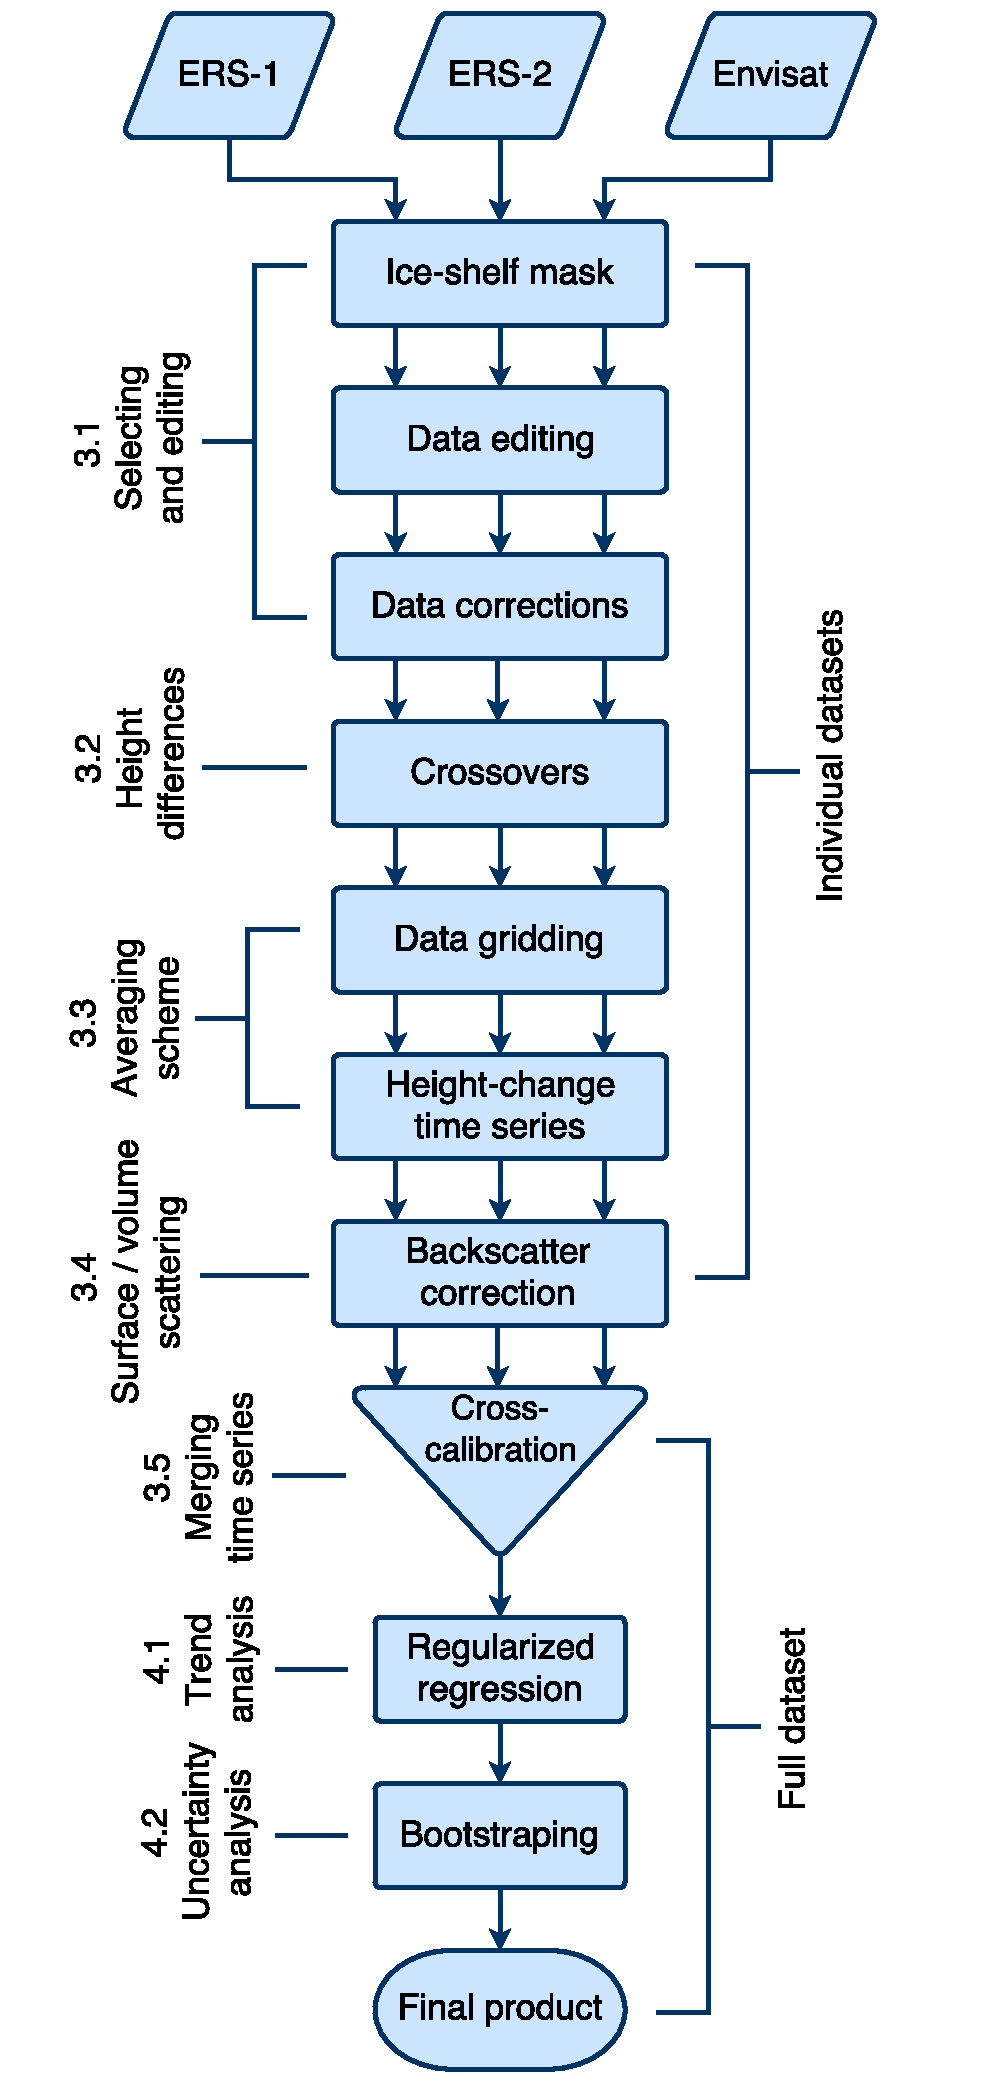
\includegraphics[width=\textwidth]{../img/flowchart_v4.pdf}
  \caption{Flowchart of our RA data processing scheme, showing the steps performed to construct an 18-year record of ice-shelf surface-height change from multiple satellite altimeters. Each step is described in Sections \ref{ra-processing} and \ref{ra-analysis}.}
  \label{c2f2}
\end{figure}

\subsubsection{Additional data corrections}

The ocean tide corrections applied to the IDR (from the CSR3 global tide model) are not accurate in Antarctica \parencite{King2005}; for that reason, we removed this correction from the data and applied an improved tide correction using the regional Circum-Antarctic Tidal Simulation model (CATS2008a), an updated version of the inverse tide model described by \parencite{Padman2002}. This tide model has higher resolution ($\sim$4 km) and a more accurate land mask than global models, resulting in more accurate tide prediction close to the coast. We also corrected for the ocean tidal loading (the elastic deformation of the seabed in response to the tide load) using the TPXO7.2 model \parencite{Egbert2002}.

\subsubsection{Estimating height differences}

To estimate the height differences at crossovers we first precisely locate the intersection points between each ascending and descending satellite track. We then find the two data points on either side of this intersection for each track pair, interpolate these to estimate the height at actual crossover location, and difference values from both tracks. When some data are missing along the satellite track, we only estimated crossover height-differences if the gap between data points on either side of the intersection point was less than 3 km. This criterion ensured that the RA pulse-limited footprints at both ends of the gap still overlapped sufficiently that interpolated heights along both tracks at the precise crossover location were consistent representations of the same location on the ice surface.

Our approach to developing time series of ice-shelf height with respect to an initial epoch $t_0$, $h(t-t_0)$, uses a multi-reference time scheme \parencite{Khvorostovsky2012, Li2006} applied to each satellite mission separately. This method computes crossover height differences for each pair of ascending and descending tracks, $\Delta h(t_i,t_j)$, throughout the entire record for a specific mission regardless of time separation between track pairs. For example, in the 9-year Envisat record, time separation of differences, $\Delta t=t_j-t_i$, at crossovers range from close to zero to nine years. 

For ERS-1, where data were acquired in different modes ('ice' and 'ocean') at different times over the ice shelves, we analyzed the crossovers $\Delta h(t_i,t_j)$ estimated from pairs of tracks with the same operation mode (ice-mode crossed with ice-mode or ocean-mode crossed with ocean-mode). Results for both modes were practically identical. In contrast, estimates of $\Delta h(t_i,t_j)$ obtained from a mixed-mode crossover (one track in ice-mode, the other in ocean-mode), were not consistent with the same-mode pairings. We also found that ice-mode data by itself was insufficient to provide near-full coverage over the ice shelves for the first few years of ERS-1 operation. Hence, for ERS-1 we retained both types of same-mode crossovers (ice-ice and ocean-ocean). For Envisat we used the fine-mode data only. 

\subsection{Averaging to enhance the signal-to-noise ratio}

For a given change in ice thickness, the estimated height-change signal over a floating ice shelf is about an order of magnitude smaller than the same signal over grounded ice. This is because, outside of a narrow ice-flexure zone roughly 1--10 km wide seaward of the grounding line, ice shelves are in hydrostatic equilibrium with a density that is about 10\% less than seawater. Since ice thickness and mass are the primary variables we wish to document, this reduced signal implies that there is a need to reduce the noise in the height estimates over ice shelves, a problem that is compounded when the goal is to identify variability over short time scales.

To enhance the signal-to-noise ratio over floating ice we implemented two averaging steps to reduce the variance in the height estimates, as described below.

\subsubsection{Spatial gridding and temporal binning}

We defined blocks of height data, $h(\mathbf{x},t_i)$, consisting of all ascending and descending tracks within non-overlapping 3-month time bins and spatial grid cells of 0.75$^\circ \times 0.25^\circ$ in longitude and latitude, respectively ($\sim30 \times 30$ km at 71$^\circ$S). At shorter time intervals, e.g., one month, the data records are often discontinuous. Aggregating data over 3-month bins provides continuous records while still resolving the annual cycle. The choice of grid-cell size ($\sim$30 km) was a compromise between characteristic spatial scales of ice-shelf processes and the spatial distribution of crossovers (Figure \ref{c2f1}). We identify each 3-dimensional block (one time bin and spatial cell), by its central time, $t_i \rightarrow i=0,1,2,..,N$, where $N$ is the total number of time bins within each satellite record, and by its central location, $\mathbf x \rightarrow 0^\circ <$ longitude $< 360^\circ$ and $-81.5^\circ <$ latitude $< -64.5^\circ$ (the center of the grid cells).

For each pair of blocks for the same cell but for separate time bins $t_i$ and $t_j$, we developed the set of all track-crossing-point height differences, ${\Delta h(t_i,t_j)}$, found by differencing all height values from the two data blocks. During this process we excluded crossover values higher than 15 m (gross outliers). For all pairs of ${t_i,t_j}$, we therefore obtained average height changes at each location as

\begin{equation}
  \overbar{\Delta h}(\mathbf{x}, t_i, t_j) = \frac{1}{n_\text{ad} + n_\text{da}} 
  \left\{
  n_\text{ad} \, \text{Md}\!\left[ \Delta h_\text{ad}(t_i, t_j) \right] +
  n_\text{da} \, \text{Md}\!\left[ \Delta h_\text{da}(t_i, t_j) \right]
  \right\}
  \label{c2e1}
\end{equation}

\noindent
where $\overbar{\Delta h}$ is the weighted-mean height-change estimate between times $t_i$ and $t_j$, $\Delta h_\text{ad}$ and $\Delta h_\text{da}$ are height changes formed by differencing ascending-descending and descending-ascending satellite ground tracks, respectively, $n_ad$ and $n_da$ are the number of crossovers of each type per block, and $\text{Md}[\,]$ is the median operator. We used the median instead of the mean because individual values of $\Delta h(t_i,t_j)$ can have large errors and its distribution can be non-Gaussian. It is necessary to use the average between ascending/descending and descending/ascending crossovers to remove any time-invariant biases, such as those introduced by the combination of satellite orientation, antenna polarization and ice surface anisotropy.

If we assume that true temporal variations in $h$ are small for small time separations (within the time bin itself, {\it i.e.}, less than three months), then the statistics of $\Delta h(t_i,t_j)$ are a measure of noise in the height difference estimates. This noise value may be spatially dependent; for example, relatively smooth and flat regions of ice shelf may have smaller noise in $\Delta h$ than regions where the ice-shelf surface is sloping or rough.

\subsubsection{Derivation of height-change time series}

The simplest way to obtain a time series of height change for a specific spatial cell is to difference the first block of data consecutively with all subsequent blocks \parencite[E.G.,]{Zwally1989}. This approach, however, results in all height differences in the resulting record being dependent upon the quality and data availability of the reference epoch (the first block). Instead, for each cell we evaluated all possible combinations between time bins within each satellite mission \parencite{Li2006}, and further combinations between the formed differences as in \textcite{Khvorostovsky2012}. This procedure was carried out as follows.

For each grid cell we constructed a set of $N-1$ time series of average height differences with respect to each of the $N-1$ separate epochs, and then formed a full matrix (one per cell) containing one height-change record per row. For example, taking $t_0$ to be the reference epoch (any time could be chosen) we then have:

\begin{equation}
  [\Delta h] = 
  \begin{pmatrix}
    h_{0,1} & h_{0,2} & h_{0,3} & \cdots & h_{0,N} \\
    -- & h_{0,1} + h_{1,2} & h_{0,1} + h_{1,3} & \cdots & h_{0,1} + h_{1,N} \\
    h_{0,2} - h_{1,2} & -- & h_{0,2} + h_{2,3} & \cdots & h_{0,2} + h_{2,N} \\
    h_{0,3} - h_{1,3} & h_{0,3} - h_{2,3} & -- & \cdots & h_{0,3} + h_{3,N} \\
    \cdots & \cdots & \cdots & \cdots & \cdots \\
    h_{0,N} - h_{1,N} & h_{0,N} - h_{2,N} & h_{0,N} - h_{3,N} & \cdots & --
  \end{pmatrix}
  \label{c2e2}
\end{equation}

\noindent
where $h_{i,j} = \overbar{\Delta h}(\mathbf{x}, t_i, t_j)$ from Eq. (\ref{c2e1}). In the example above, every row constitutes a time series of height change with respect to $t_0$. This is accomplished by (i) forming the upper triangle of the matrix from the calculated average differences, (ii) forming the lower triangle as the negative of the upper one, and (iii) using the elements of the first row (time series with respect to $t_0$) to reference each of the other rows (Figure \ref{c2f3}). We note that any row in the matrix could be used as the reference series ({\it i.e.}, any epoch); the optimal one, however, will cover the largest time span in the presence of data gaps.

Next, we weight-averaged the matrix rows by the number of crossovers used to form each average difference to produce a mean time series per cell, with reduced statistical error:

\begin{equation}
  h(\mathbf x, \tau) = \langle [\Delta h] \rangle 
  \label{c2e3}
\end{equation}

\noindent
where $\tau = t - t_0$. We propagated individual errors in the averaging procedure assuming normality \parencite{Li2006}.

To evaluate possible signal aliasing we used a small region to test aggregating data in 3-month bins that were overlapped by $1/3$ as in \textcite{Khvorostovsky2011}. The overlapping approach required a much longer computation time, and the resulting average time series were the same as the non-overlapping approach, and so we did not apply this to the full dataset.


\begin{figure}[!ht]
  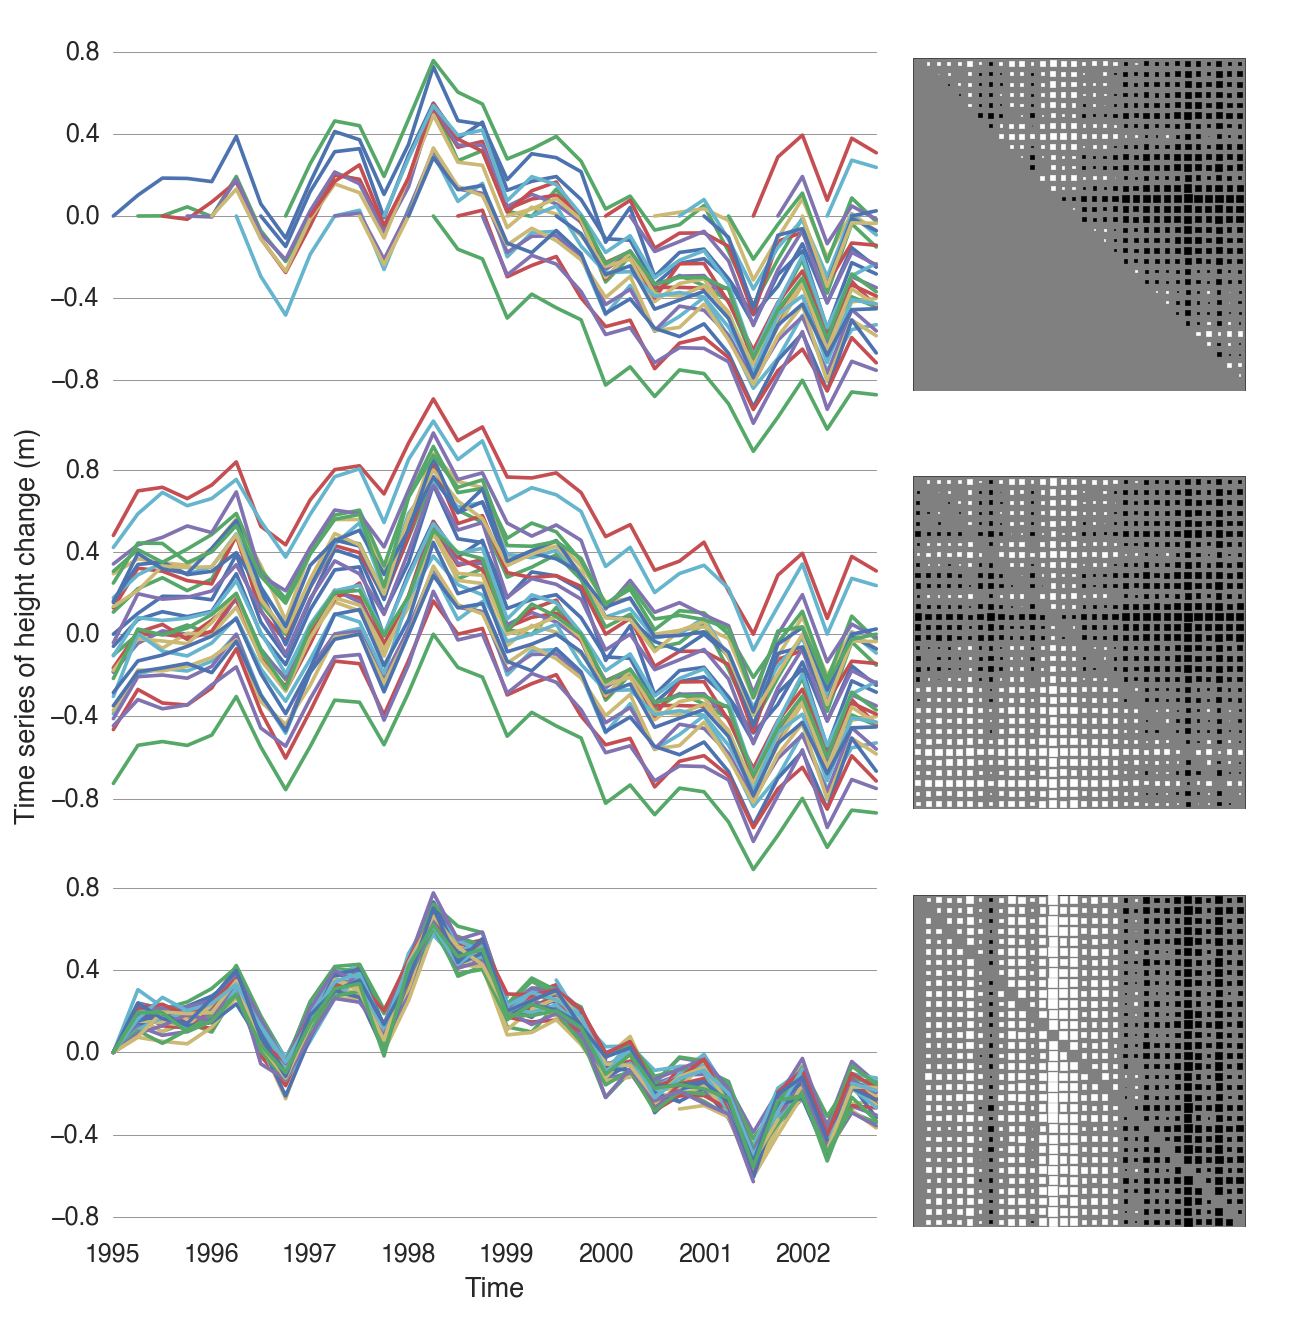
\includegraphics[width=\textwidth]{../img/multiref_matrix_v4.png}
  \caption{
  Representation of the multi-reference time series approach. (left) Individual time series of cumulative change. (right) Diagram representing the matrix formed with the time series on the left (one time series per row). From top to bottom is depicted the process of forming single-grid-cell average time series: (top) the one-sided matrix of average differences; (middle) the two-sided matrix; (bottom) referencing all the rows (time series) to a common epoch for posterior averaging (this matrix is Eq. \ref{c2e2}).} 
  \label{c2f3}
\end{figure}

\subsection{Surface and volume scattering variation}

Interpreting heights derived from RA data over snow-covered ice surfaces requires an understanding of the complex interaction of the radar wave with the snowpack and firn (compressed snow that has not yet formed into solid ice). Over ice sheets, part of the incident radar energy penetrates into the snowpack/firn \parencite{Ridley1988} by an amount that depends on the properties of the surface layers including temperature, density, grain-size and moisture content \parencite{Davis1993}, leading to volume scattering with reflections within sub-surface layers and ice lenses. Volume scattering increases the path length of the radiation and, therefore, its travel-time back to the satellite and the inferred height. The waveform shape in the presence of volume scattering is also different than if only surface scattering occurred. In some cases, most of the echo can be from a well-defined sub-surface horizon within the snowpack \parencite{Thomas2008}, leading to a surface-like waveform shape, but a height estimate that is still lower than the true surface.

The penetration depth (where the radar pulse decays by $1/e$ of its initial intensity) varies with density, grain-size, and water content of the snow/firn. Penetration depth can be several meters over the colder and dryer parts of the Antarctic plateau where grain sizes are smaller but is much lower (on the order of centimeters) over the warmer and wetter ice shelves where grain sizes are larger \parencite{Davis1996}. To demonstrate this we used the \parencite{Davis1993} surface/volume algorithm to estimate the extinction coefficient ($k_\text{e}$; which is inversely proportional to penetration depth) for the entire Antarctic area under the ERS-1 satellite's coverage, using ERS-1 altimeter level-1 ocean-mode waveforms (Phase C) (Figure \ref{c2f4}). In general, $k_\text{e}$ is on the order of 4--5 times higher over the ice shelves than elsewhere on the ice sheet. This means that the penetration bias is not as large over the ice shelves as it is over the ice sheet interior.

The return radar waveform used to estimate the surface height is the sum of surface echo (energy scattered by the surface) and volume echo (energy scattered within the snowpack). Perturbations in the return radar waveform occur by changes in the properties of the snowpack, which alters the effective backscatter layer, potentially leading to a biased surface-height estimate. Two competing effects (with opposite signs) play a significant role in altering the shape of the return waveform: i) penetration of the signal into the firn layer increases volume scattering (increasing the waveform’s leading-edge width); and ii) densification of the surface increases the air-snow dielectric contrast (decreasing the leading-edge width). We investigated corrections to minimize these effects as described in Section \ref{bs-corr} below.


\begin{figure}[!ht]
  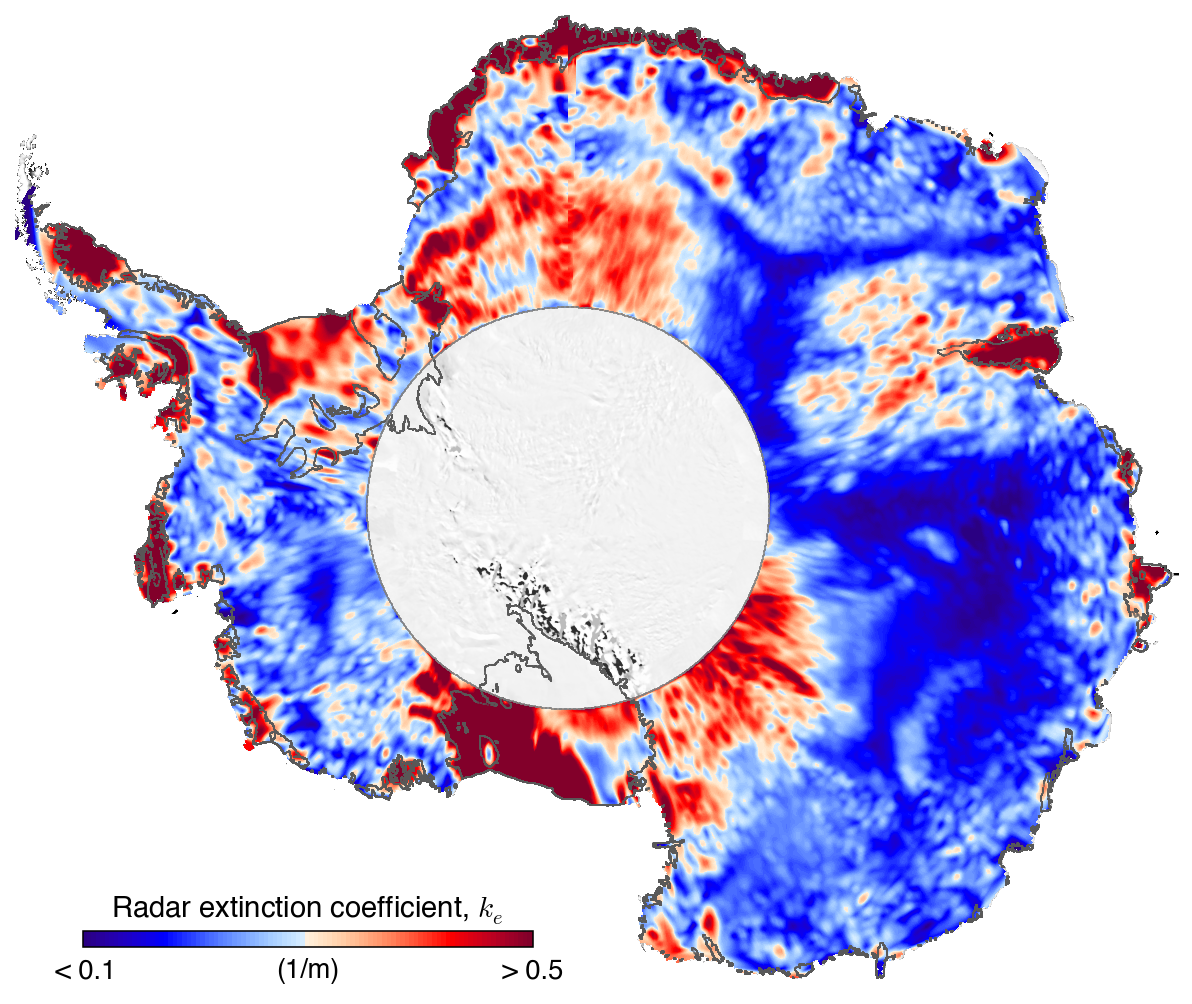
\includegraphics[width=\textwidth]{../img/extinction_coef_v3d.png}
  \caption{
  Estimated radar altimeter extinction coefficient ($k_\text{e}$) over the Antarctic ice sheet. $k_\text{e}$ was derived from ERS-1 Phase C ocean-mode return waveforms over the ice sheet and ice shelves using a surface/volume scattering algorithm \parencite{Davis1993}. Note that the $k_\text{e}$  (which is inversely related to the penetration depth) is generally higher in the ice shelves than on the plateau. This difference can mostly be explained in terms of grain sizes: on the ice shelf, individual particles are larger than those on the plateau, due to much warmer temperatures, combined with successive melt-freeze cycles ({\it i.e.}, wet snow metamorphosis) \parencite{Zwally1994}; therefore $k_\text{e}$ is high. On the plateau, grain sizes depend on surface temperature and accumulation rate. In general, as elevation and distance from the coast (continentally) increases, temperatures decrease; therefore the grain sizes and $k_\text{e}$ decrease.
  }
  \label{c2f4}
\end{figure}

\subsubsection{Correction for changes in backscatter}
\label{ra-corr}

Although much progress has been made in understanding the relation between backscatter fluctuation, resulting mainly from variations in near-surface properties, and altimeter-derived height \parencite{Arthern2001, Davis1993, Legresy1998, Partington1989, Remy2012, Ridley1988}, it is still an active area of investigation and its full impact on the RA measurement error remains poorly known \parencite{Remy2012}. To attempt to minimize the impact on the estimated height of fluctuations in backscatter, an empirical adjustment using backscatter information is performed \parencite{Davis2004, Khvorostovsky2012, Remy2009, Wingham2006, Wingham1998, Zwally2005}.

We used the altimeter automatic gain control (AGC) as a measure of backscattered power to adjust our height-change time series using corresponding series of changes in AGC, $g(\mathbf x,\tau)$. We formed these backscatter-change time series for each grid cell in the same way as the height-change series described above. We derived a spatially variant sensitivity factor, $S(\mathbf x)$, to scale the backscatter values at each grid-cell. This sensitivity is the regression slope of the correlation between height and backscatter changes that we derived independently for each RA mission. We then corrected each time series as follows:

\begin{equation}
  h(\mathbf x,\tau)_\text{cor} = h(\mathbf x,\tau) 
    - S(\mathbf x) \, g(\mathbf x,\tau) - h_0(\mathbf x)
  \label{c2e4}
\end{equation}

\noindent
where $h_\text{cor}$ is backscatter-corrected height-change, $S$ is the sensitivity factor (altimeter dependent), $g$ is gain change, and $h_0$ is the regression intercept (not needed for correcting full independent records relative to some epoch). For the regression procedure we used a robust method, M-estimator \parencite{Huber1981}, instead of the commonly used least-squares approach, which can be sensitive to outliers (especially when few data are available).

In selecting an optimal backscatter correction scheme we tested three different approaches. We correlated series of backscatter and height changes: i) using the cross-calibrated full 18-year records, ii) using data within 2 and 3-year sliding windows (similar to \textcite{Khvorostovsky2012}) and iii) using independent single-mission records. For each approach we performed the correlation using both the original time series (absolute values) and the differenced series (derivative). We found that the third approach was the only one to perform consistently under a variety of conditions ({\it e.g.}, high vs. low variance, high vs. low correlation, high vs. low heteroscedasticity). Note that using differenced series is equivalent to using high-pass filtered records and, therefore, higher correlations are expected since backscatter change is primarily a function of seasonality. However, in correlating differenced series only the short-term fluctuations in backscatter are being taken into account. Hence, we corrected our height-change records by correlating series of absolute values using (iii).

\subsubsection{Densification from changes in the firn column}

One approach to accounting for changing surface mass balance over an ice shelf, specifically firn compaction/densification, is to use an atmospheric-based model to predict how the firn column evolves under modeled climate conditions. For example, a laser altimeter study by \textcite{Pritchard2012} used modeling of changes in the firn column to isolate the part of the signal due to fluctuations in the snowpack. We performed a correlation analysis between our backscatter-uncorrected time series, which contain the seasonal response of the ice-shelf surface as detected by the altimeter's automatic gain control (backscatter), and the height changes derived from a firn densification model (FDM). To construct the firn height-change record we used the \textcite{Ligtenberg2011}’s FDM from which (i) we extracted firn height-change series for each location in our grid; (ii) averaged the 48-hour firn records with a 3-month moving window; and (iii) retained the discrete time-values that corresponded to our 3-month ice-shelf height records.

We found no correlation between the firn height changes and RA-derived changes in ice-shelf height at the fine resolution required for this study (individual grid cells of $\sim$30 km). The firn model was able to provide, however, an estimate of the expected seasonal variation of the firn height at the larger scale (Figure \ref{c2f5}). Additionally, since some degree of penetration through fresh snow is expected at the frequency of the Ku-band altimeter, satellite RAs are less sensitive than are laser altimeters to fluctuations in surface mass balance. For these reasons we found no justification to use a FDM to make any firn-change correction on RA height estimates.


\begin{figure}[!ht]
  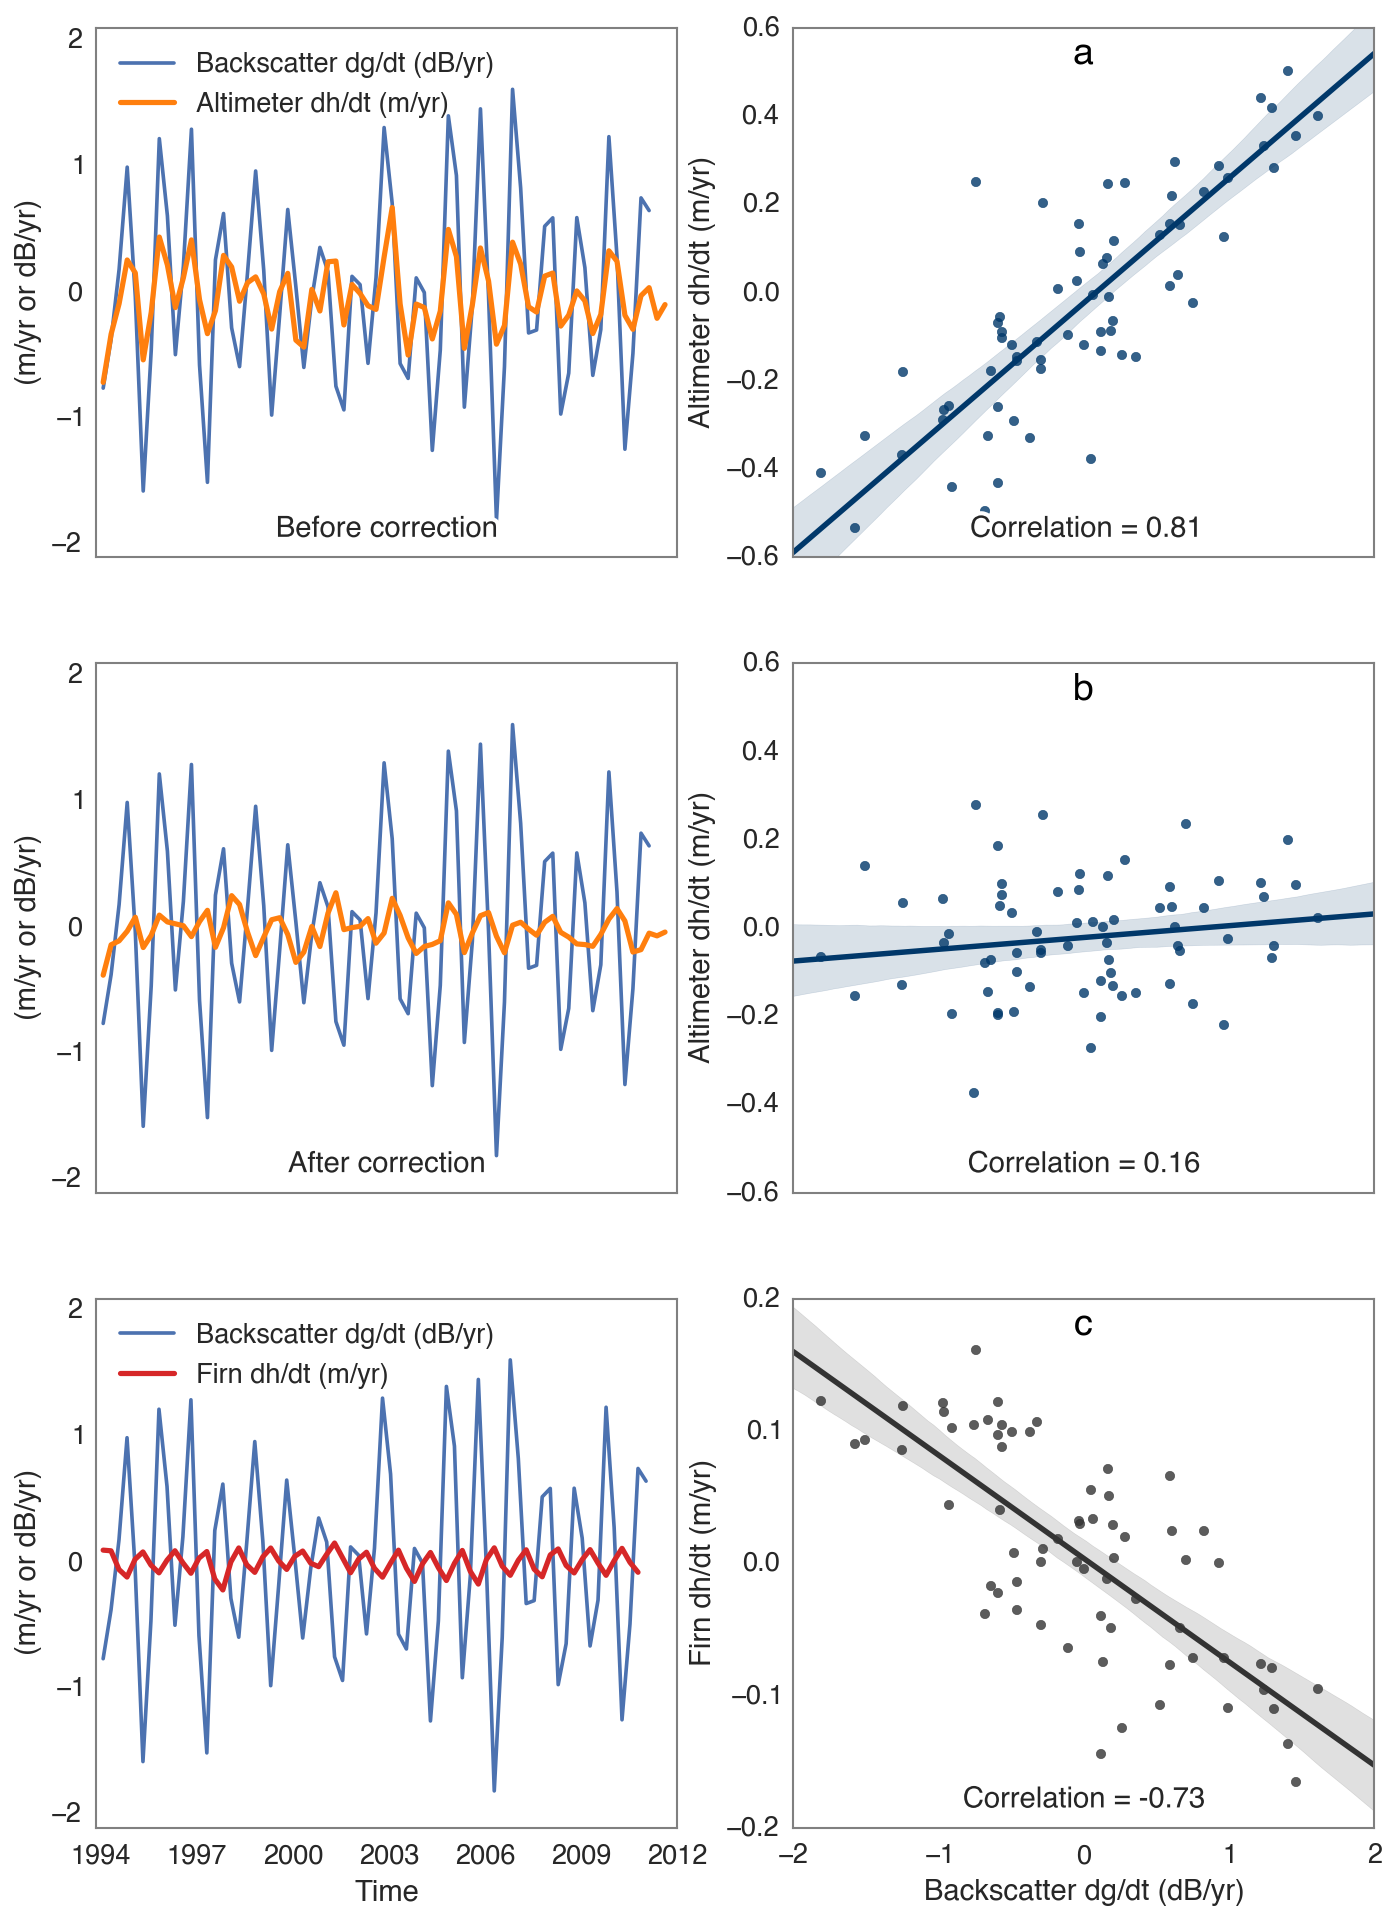
\includegraphics[width=\textwidth]{../img/correlation_h_b_f_v7.png}
  \caption{
  Correlation between backscatter (AGC), ice-shelf height and firn-height change derived from a firn densification model. (left column) Derivative of circum-Antarctic-wide average time series; (right column) respective correlations. From top to bottom, correlations between the derivative of backscatter and derivatives of: (a) uncorrected ice-shelf height; (b) corrected ice-shelf height (at the grid-cell level); and (c) firn-column height time series.
  } 
  \label{c2f5}
\end{figure}



\printbibliography[segment=2,heading=subbibliography]


% Chapter 3 - Trend Analysis 
% --------------------------
% Jun 1, 2015


\chapter{Trend analysis of ice-shelf height}

{\sl
\noindent
This chapter, in full, is a reprint of:\\
Volume loss from Antarctic ice shelves is accelerating, F.\,S.~Paolo, H.\,A.~Fricker, L.~Padman, {\rm Science} (2015). doi:10.1126/science.aaa0940
}

\section{Abstract}

The floating ice shelves surrounding the Antarctic Ice Sheet restrain the
grounded ice-sheet flow. Thinning of an ice shelf reduces this effect, leading
to an increase in ice discharge to the ocean. Using 18 years of continuous
satellite radar altimeter observations, we have computed decadal-scale changes
in ice-shelf thickness around the Antarctic continent. Overall, average
ice-shelf volume change accelerated from negligible loss at 25 $\pm$ 64 cubic
kilometers per year for 1994--2003 to rapid loss of 310 $\pm$ 74 cubic
kilometers per year for 2003--2012. West Antarctic losses increased by
$\sim$70\% in the past decade, and earlier volume gain by East Antarctic ice
shelves ceased. In the Amundsen and Bellingshausen regions, some ice shelves
have lost up to 18\% of their thickness in less than two decades.

\section{Introduction}

The Antarctic Ice Sheet gains mass through snowfall and loses
mass at its margin through submarine melting and iceberg calving. These losses
occur primarily from ice shelves, the floating extensions of the ice sheet.
Antarctica's grounded-ice loss has increased over the past two decades
\parencite{Shepherd2012, Sutterley2014}, with the most rapid losses being along
the Amundsen Sea coast \parencite{Joughin2011} concurrent with substantial
thinning of adjoining ice shelves \parencite{Shepherd2010, Pritchard2012} and
along the Antarctic Peninsula after ice-shelf disintegration events \parencite{
Scambos2004}. Ice shelves restrain ("buttress") the flow of the grounded ice
through drag forces at the ice-rock boundary, including lateral stresses at
sidewalls and basal stresses where the ice shelf rests on topographic highs
\parencite{Schoof2007, Goldberg2009}. Reductions in ice-shelf thickness reduce
these stresses, leading to a speed-up of ice discharge. If the boundary between
the floating ice shelf and the grounded ice (the grounding line) is situated on
a retrograde bed (sloping downwards inland), this process leads to faster rates
of ice flow, with potential for a self-sustaining retreat \parencite{
Schoof2007, Favier2014, Joughin2014}.

Changes in ice-shelf thickness and extent have primarily been attributed to
varying atmospheric and oceanic conditions \parencite{Scambos2003, Dutrieux2014}.
Observing iceshelf thickness variability can help identify the principal 
processes influencing how changing large-scale climate affects global sea level
through the effects of buttressing on the Antarctic Ice Sheet. The only
practical way to map and monitor ice-shelf thickness for this vast and remote
ice sheet at the known space and time scales of ice-shelf variability is with
satellite altimetry. Previous studies have reported trends based on simple line
fits to time series of ice-shelf thickness (or height) averaged over entire ice
shelves or broad regions \parencite{Shepherd2010, Zwally2005} or for short 
($\sim$5-year) time intervals \parencite{Pritchard2012, Rignot2013,Depoorter2013}.
Here, we present a record of ice-shelf thickness that is highly resolved in 
time ($\sim$3 months) and space ($\sim$30 km), using the longest available 
record from three consecutive overlapping satellite radar altimeter missions
(ERS-1, 1992--1996; ERS-2, 1995--2003; and Envisat, 2002--2012) spanning 18
years from 1994 to 2012.


\section{Methods}

Our technique for ice-shelf thickness change detection is based on crossover
analysis of satellite radar altimeter data, in which time-separated height 
estimates are differenced at orbit intersections \parencite{Zwally2005, 
Davis2004, Wingham2009}. To cross-calibrate measurements from the different 
satellite altimeters, we used the roughly 1-year overlap between consecutive
missions. The signal-to-noise ratio of altimeter-derived height differences for
floating ice in hydrostatic equilibrium is roughly an order of magnitude 
smaller than over grounded ice, requiring additional data averaging to obtain
comparable statistical significance. We aggregated observations in time 
(3-month bins) and space ($\sim$30-km cells). Because the spatial distribution
of crossovers changes with time (due, for example, to non-exact repeat tracks
and nadir mispointing), we constructed several records at each cell location
and stacked them in order to produce a mean time series with reduced
statistical error\footnote{\label{SM}Materials and methods are available as 
supplementary materials on {\it Science} Online, and reproduced in part at the end of
this chapter and the majority of it in {\sl Chapter 2}.}. We converted our height-change time series and rates to
thickness changes by assuming that observed losses occurred predominantly at
the density of solid ice (basal melting) \parencite{Shepherd2010,
Pritchard2012, Wingham2009}. This is further justified by the relative
insensitivity of radar measurements to fluctuations in surface mass 
balance\footnotemark[1]. For volume changes, we tracked the minimum (fixed) area of
each ice shelf\footnotemark[1]. We assessed uncertainties for all estimates using
the bootstrap approach (resampling with replacement of the residuals of the
fit) \parencite{Efron1993}, which allows estimation of formal confidence
intervals. All our uncertainties are stated at the 95\% confidence level 
(discussion of uncertainties are provided in [\footnotemark[1]] and the several
corrections applied are stated in [\footnote{Corrections include lag of the
satellite's leading-edge tracker (retracking), surface scattering variations,
surface slope, dry atmospheric mass, water vapor, the ionosphere, solid Earth
tide, ocean tide and loading, atmospheric pressure, and regional sea-level
variation\footnotemark[1].}]).

We estimated 18-year trends in ice-shelf thickness by fitting low-order 
polynomials (degree n $\leqslant$ 3) to the data using a combination of lasso
regularized-regression \parencite{Tibshirani1996} and cross-validation for
model-parameter selection (the shape of the fit is determined by the data).
This combined approach allowed us to minimize the effect of short-term
variability on the 18-year trends. Relative to previous studies
\parencite{Shepherd2010, Pritchard2012, Zwally2005, Fricker2012}, we have
improved estimations by (i) using 18-year continuous records, (ii) implementing
a time series averaging scheme so as to enhance the signal-to-noise ratio, and
(iii) using a robust approach to trend extraction.

\section{Results and discussion}

The 18-year average rate of thickness change varies spatially (Fig.~\ref{fig:ice-shelf-change}).
On shorter time scales, trends are highly variable but spatially coherent
(Fig.~\ref{fig:ice-shelf-var} and movie\footnote{\url{https://www.youtube.com/watch?v=ii8enEyfFlo}}). We divided our data set into eight regions on the basis of spatial coherence of long-term
ice-shelf behavior and calculated time series of ice-shelf thickness change
(relative to series mean) for each region (Fig.~\ref{fig:ts-regions}). The largest regional
thickness losses were in the Amundsen and Bellingshausen seas, with average
(and maximum) thinning rates of 19.4 $\pm$ 1.9 (66.5 $\pm$ 9.0) m/decade and
7.4 $\pm$ 0.9 (64.4 $\pm$ 4.9) m/decade, respectively. These values correspond
to $\sim$8 and 5\% of thickness loss over the 18 years for the two regions,
respectively. These two regions account for less than 20\% of the total West
Antarctic ice-shelf area but, combined, contribute more than 85\% of the total
ice-shelf volume loss from West Antarctica. The area-averaged time records of
ice-shelf thickness and volume for the West and East Antarctic sectors 
(Fig.~\ref{fig:ice-shelf-change}, bottom left), broad regions (Fig.~\ref{fig:ts-regions}), and single ice
shelves (Fig.~\ref{fig:ts-ice-shelves-wais} and \ref{fig:ts-ice-shelves-eais}) at 3-month time intervals show a wide range of
temporal responses with large interannual-to-decadal fluctuations, stressing
the importance of long records for determining the long-term state of the ice
shelves. Comparing our long records with simple linear trends obtained for the
periods of single satellite missions (such as the 5-year ICESat time span used
in \textcite{Pritchard2012}) shows that it is often not possible to capture the
persistent signals in the shorter records (Fig.~\ref{fig:ts-regions}, \ref{fig:ts-ice-shelves-wais} and \ref{fig:ts-ice-shelves-eais}).


\begin{figure}[!h]
  \centering
  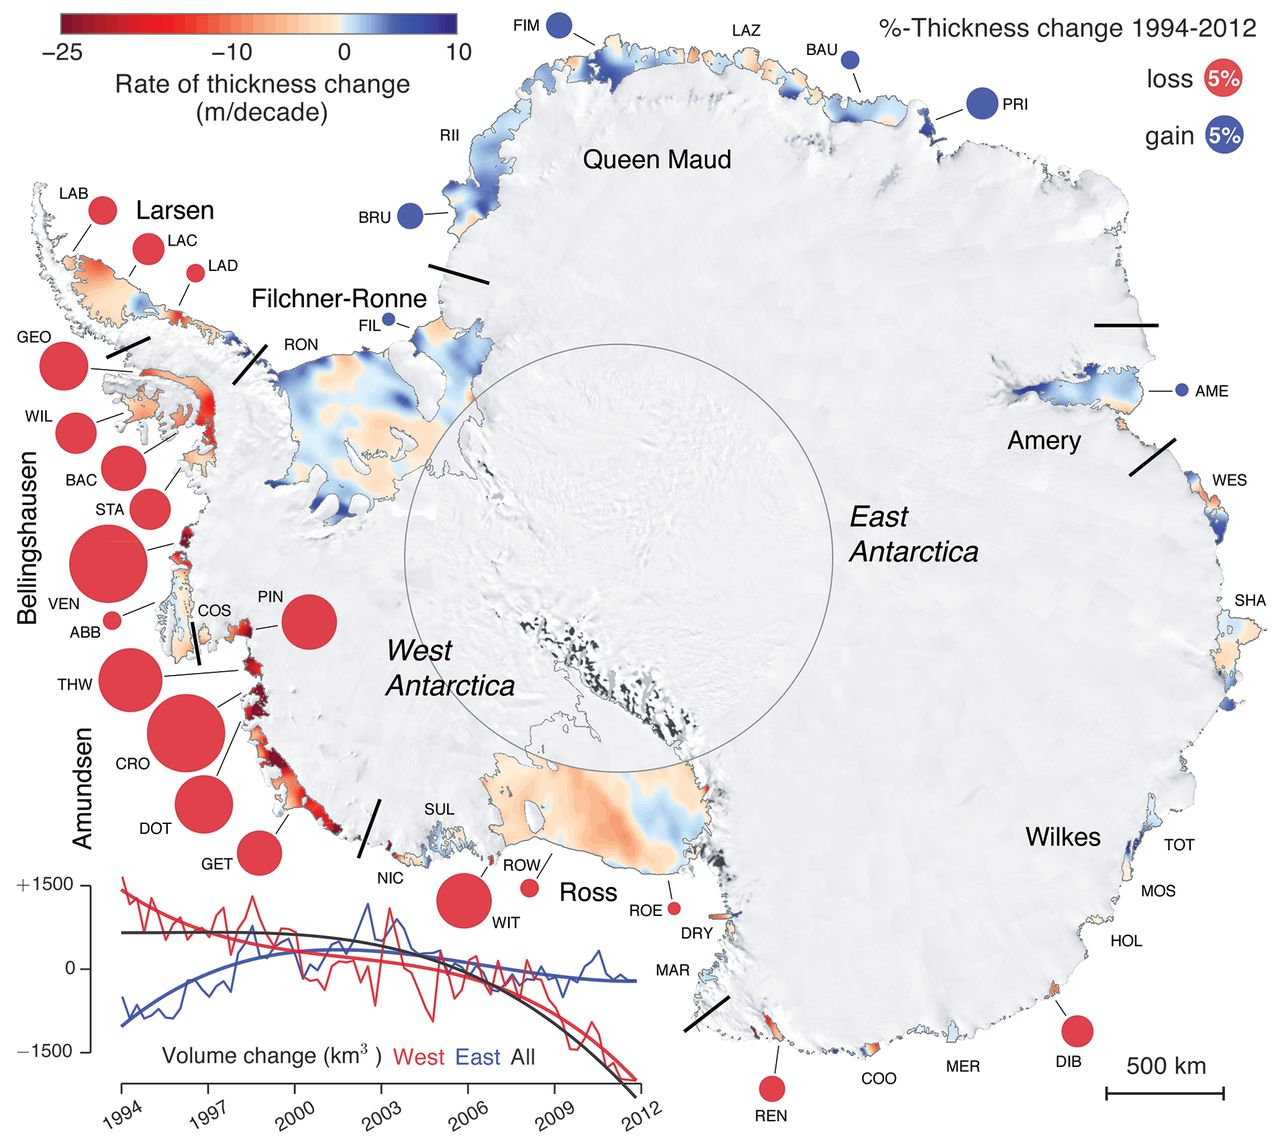
\includegraphics[width=\textwidth]{img/Fig1_dzdt_map_final.jpg}
  \caption[Eighteen years of change in thickness and volume]{
  \ssp \footnotesize
  Eighteen years of change in thickness and volume of Antarctic
  ice shelves. Rates of thickness change (meters per decade) are colorcoded
  from $-$25 (thinning) to $+$10 (thickening). Circles represent percentage of
  thickness lost (red) or gained (blue) in 18 years. Only significant values at
  the 95\% confidence level are plotted (Table \ref{tab:estimates}). (Bottom left)
  Time series and polynomial fit of average volume change (cubic kilometers)
  from 1994 to 2012 for the West (in red) and East (in blue) Antarctic ice
  shelves. The black curve is the polynomial fit for All Antarctic ice shelves.
  We divided Antarctica into eight regions (Fig.~\ref{fig:ts-regions}), which are labeled
  and delimited by line segments in black. Ice-shelf perimeters are shown as a
  thin black line. The central circle demarcates the area not surveyed by the
  satellites (south of 81.5\degree S). Original data were interpolated for
  mapping purposes (percentage area surveyed of each ice shelf is provided in
  Table \ref{tab:estimates}). Background is the Landsat Image Mosaic of Antarctica
  (LIMA).}
  \label{fig:ice-shelf-change}
\end{figure}
\clearpage


\begin{figure}[!h]
  \centering
  \vspace{1.2cm}
  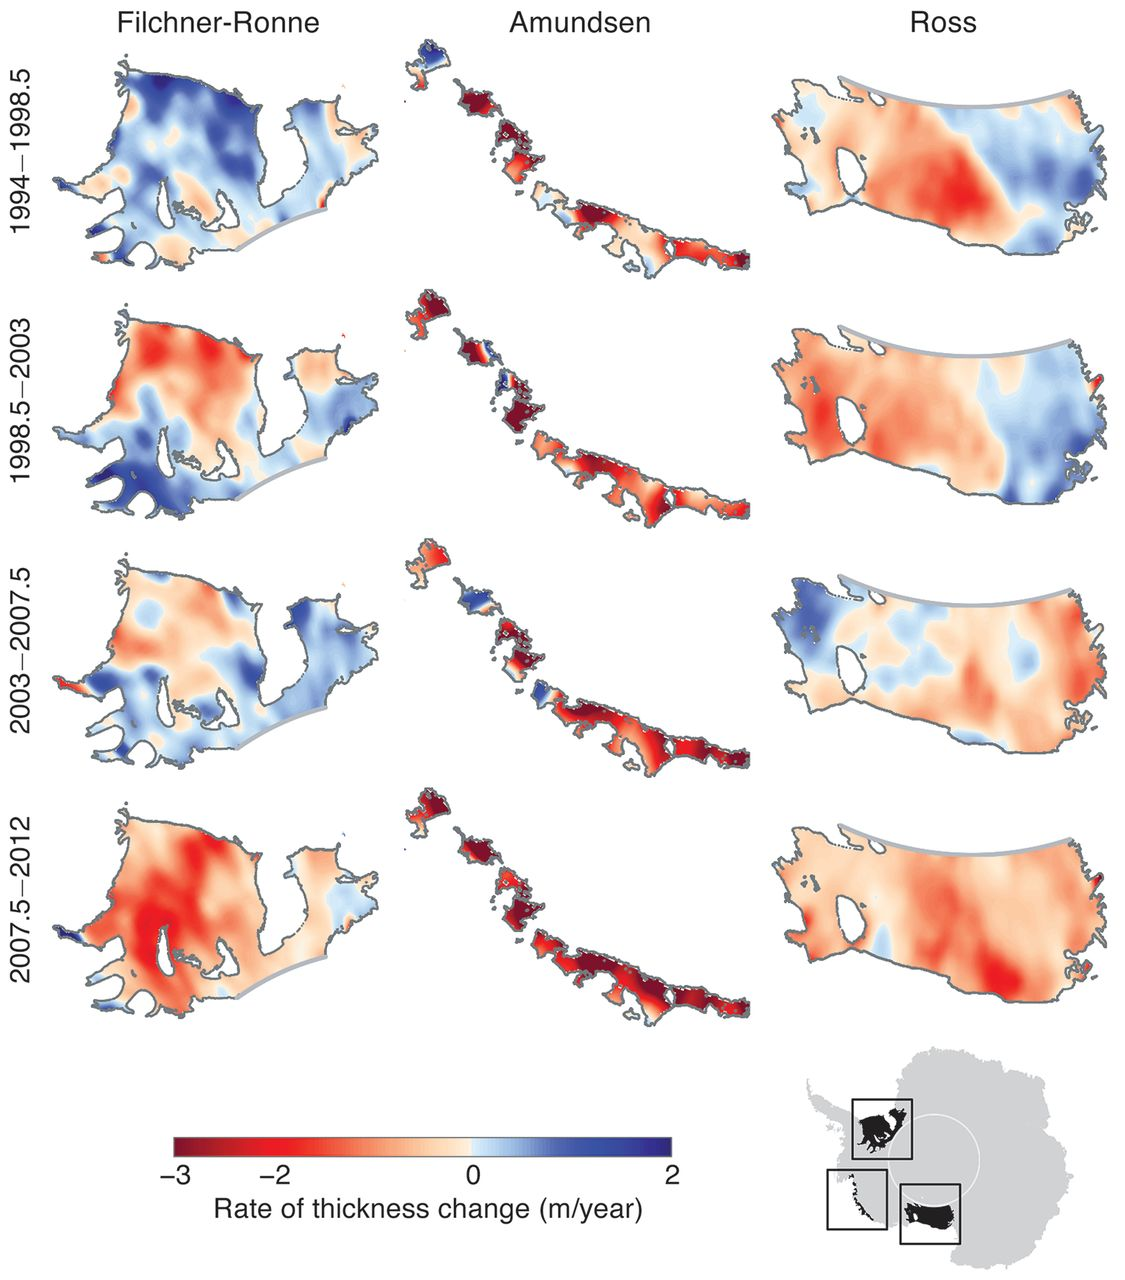
\includegraphics[width=.95\textwidth]{img/Fig2_pannels_review_final.jpg}
  \vspace{.8cm}
  \caption[Variability in the rate of Antarctic ice-shelf thickness]{
  \ssp \footnotesize
  Variability in the rate of Antarctic ice-shelf thickness change
  (meters per year). Maps for (columns from left to right) Filchner-Ronne,
  Amundsen,and Ross ice shelves (locations in the bottom right corner) showing
  average rate of thickness change for (rows) four consecutive 4.5-year
  intervals (1994--1998.5, 1998.5--2003, 2003--2007.5, and 2007.5--2012).
  Shorter-term rates can be higher than those from an 18-year interval.
  Ice-shelf perimeters are thin black lines, and the thick gray line demarcates
  the limit of satellite observations.}
  \label{fig:ice-shelf-var}
\end{figure}
\clearpage


\begin{figure}[!h]
  \centering
  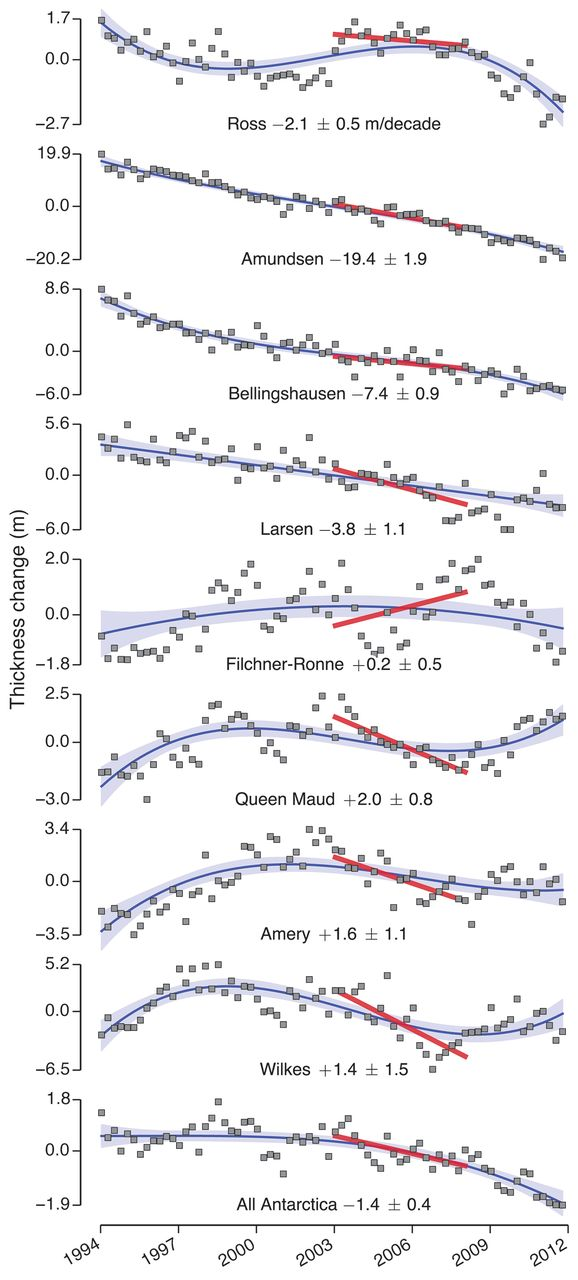
\includegraphics[width=.53\textwidth]{img/Fig3_ts_regions_review_final.jpg}
  \caption[Time series of cumulative thickness change]{
  \ssp \footnotesize
Time series of cumulative thickness change relative to series mean for Antarctic ice-shelf regions (1994--2012). Time series correspond to averages for all ice-shelf data within the Antarctic regions defined in Fig.~\ref{fig:ice-shelf-change}. Dots represent average thickness change every 3 months. Error bars are small (in many cases, smaller than the symbols themselves, thus omitted from the plots), making the interannual fluctuation shown by the dots significant. The blue curve is the long-term trend from polynomial regression with the 95\% confidence band, and the red line shows the regression line to the segment of our data set that overlaps with the period used for a prior ICESat-based analysis (2003--2008) \parencite{Pritchard2012}. Average rates (in meters per decade) are derived from the end points of the polynomial models.
  \label{fig:ts-regions}
  }
\end{figure}


Ice-shelf average thinning rates from the 18-year polynomial fits in the
Amundsen Sea region (AS) range from 1.5 $\pm$ 0.9 m/decade for Abbot to 
31.1 $\pm$ 5.4 m/decade for Crosson, with local maximum thinning of 
66.5 $\pm$ 9.0 m/decade on Getz (Fig.~\ref{fig:ts-ice-shelves-wais} and Table
\ref{tab:estimates}). Crosson and Getz have lost $\sim$18 and 6\% of their
thicknesses, respectively, over the 18-year period. If this thinning persists
for these two ice shelves, we can expect volume losses of $\sim$100 and 30\%,
respectively, in the next 100 years. Getz is the single largest contributor to
the overall volume loss of Antarctic ice shelves, with an average change of 
$-$54 $\pm$ 5 km$^3$/year, accounting for $\sim$30\% of the total volume loss
from the West Antarctic ice shelves (Table \ref{tab:estimates}). We find the most
dramatic thickness reduction on Venable Ice Shelf in the Bellingshausen Sea
(BS), with an average (and maximum) thinning rate of 36.1 $\pm$ 4.4
(64.4 $\pm$ 4.9) m/decade, respectively (Fig.~\ref{fig:ts-ice-shelves-wais} and Table
\ref{tab:estimates}). This ice shelf has lost 18\% of its thickness in 18 years,
which implies complete disappearance in 100 years.

For the ice shelves in the AS, observed rates
are highest near the deep grounding lines, with
lower rates found toward the shallower ice fronts
(Fig.~\ref{fig:ice-shelf-var}, Table \ref{tab:estimates}, and movie\footnote{\url{https://www.youtube.com/watch?v=ii8enEyfFlo}}). This pattern is
consistent with enhanced melting underneath
the ice shelf forced by an increased flux of circumpolar
deep water (CDW) from across the continental
shelf and into the sub-ice-shelf cavity
\parencite{Dutrieux2014, Jacobs2011, Thoma2008}. The consequent loss of ice-shelf buttressing
from increased ocean-forced melting may
have driven the grounding lines inland \parencite{Rignot2014} to
a point on a retrograde bed slope at which the
marine ice-sheet instability mechanism can take
over the dynamics of ice export \parencite{Schoof2007, Weertman1974}. Hence,
observed ice-shelf thinning reflects both ocean-induced
basal melting and increased strain rates
resulting from faster flows. Our analysis shows
that thinning was already under way at a substantial
rate at the start of our record in 1994.

On the eastern side of the Antarctic Peninsula
[comprising Larsen B (Scar Inlet remnant), Larsen 
C, and Larsen D], the regional ice-shelf thinning
rate of 3.8 $\pm$ 1.1 m/decade (Fig.~\ref{fig:ts-regions}) is about half of
that on the western side (BS) (Fig.~\ref{fig:ice-shelf-change}). The onset of
thinning for Larsen C has progressed southward
(Fig.~\ref{c3f4}), which is consistent with climate-driven
forcing discussed in earlier studies \parencite{Fricker2012, Cook2010}. The
highest thinning rates on Larsen C (with local
maximum thinning of 16.6 $\pm$ 8.1 m/decade) are
near Bawden Ice Rise (Fig.~\ref{fig:ice-shelf-change}~and~\ref{c3f4}). Assuming
that half of this observed thinning is due to air
loss within the firn column, and considering
that the ice shelf is $\sim$40 m above flotation over
the ice rise \parencite{Holland2015}, we can expect Larsen C to fully
unground from this pinning point within the
next 100 years, with potential consequences on
the ice-shelf stability \parencite{Borstad2013}.


\begin{figure}[!h]
  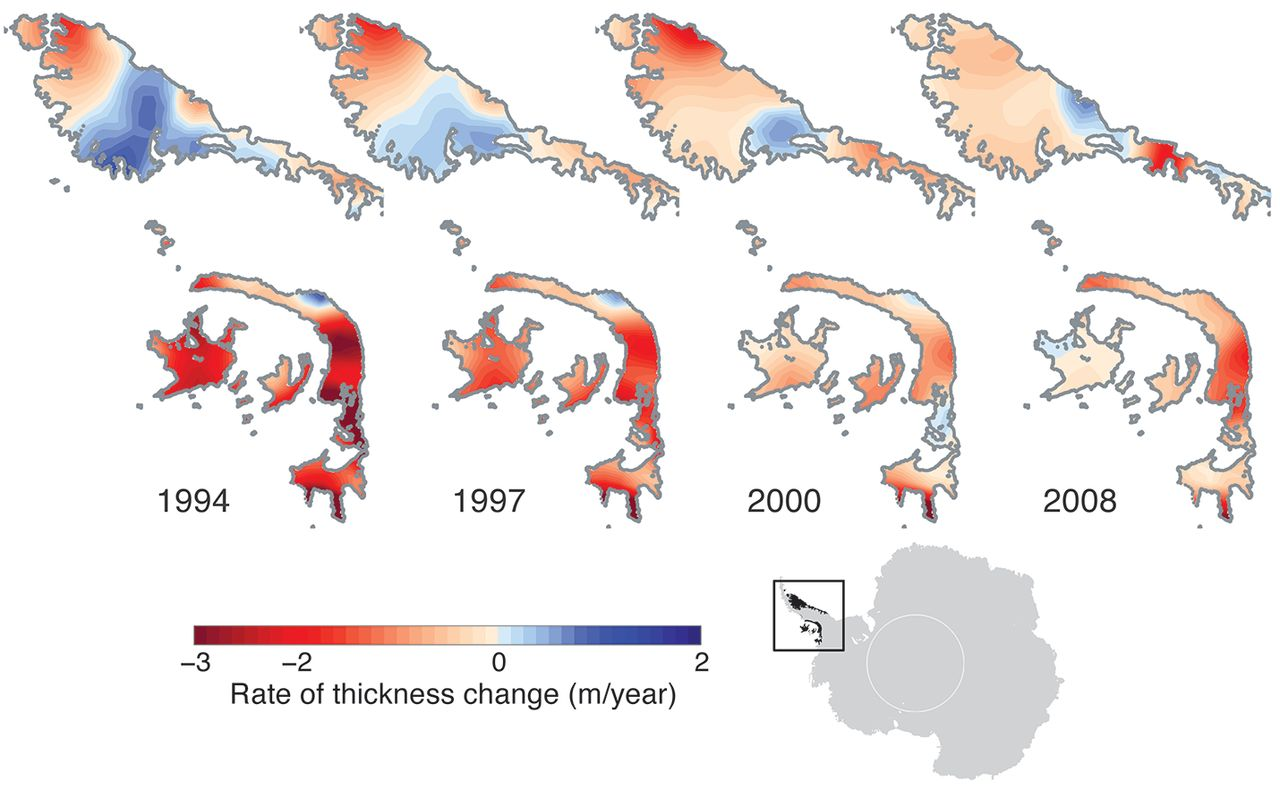
\includegraphics[width=\textwidth]{img/Fig4_antpen_pannels_review_final.jpg}
  \caption[Evolution of the rate of thickness change]{
  \ssp \footnotesize
  Evolution of the rate of thickness
  change in the Antarctic Peninsula. Instantaneous
  rate-of-thickness change (meters per year) for
  four specific times (1994, 1997, 2000, and 2008)
  is calculated as the derivative of the polynomial fit
  to the thickness-change time series. The rate
  increases spatially with time from north to south
  in the Larsen Ice Shelf (see movie\footnote{\url{https://www.youtube.com/watch?v=ii8enEyfFlo}}). The eastern
  (Weddell Sea) side of the Antarctic Peninsula (top)
  shows independent behavior from the western
  (Bellingshausen Sea) side (bottom).
  }
  \label{c3f4}
\end{figure}


The regional time-varying trends for the ice
shelves in the three East Antarctic regions (Queen
Maud, Amery, and Wilkes) are coherent (Fig.~\ref{fig:ts-regions}).
Ice shelves in the Wilkes region are challenging
for conventional radar altimeters because many
of them are small, contained in narrow embayments,
and have rough surfaces so that altimeter-derived
height changes do not necessarily reflect
thickness change accurately. Our estimate of overall
thickness change for the Wilkes ice shelves is
1.4 $\pm$ 1.5 m/decade, which is not significantly
different from zero. The Queen Maud region ice
shelves show an overall increase in thickness of
2.0 $\pm$ 0.8 m/decade.

Like the AS ice shelves, Totten and Moscow
University ice shelves in the Wilkes region buttress
a large marine-based section of the East
Antarctic ice sheet so that their stability is potentially
important to grounded-ice loss. Although
these ice shelves were previously reported as
thinning \parencite{Pritchard2012} on the basis of a straight-line fit to
a 5-year record from a satellite laser altimeter
(ICESat, 2003--2008), our results show that those
estimates are not representative of the longer-term
trends (Fig.~\ref{fig:ts-ice-shelves-eais}). Our estimate of thickness
loss during 2003--2008 is similar to the ICESat-based
result, but the full 18-year period shows
thickness trends that are not significantly different
from zero (Fig.~\ref{fig:ts-ice-shelves-eais}).

For most ice shelves, our estimates are significantly
different from previous results (Table \ref{tab:comparison}).
Several factors contribute to this. (i) The areas of
ice shelves over which measurements are averaged
vary between studies, affecting estimates on
small ice shelves with large thickness-change
signals. (ii) Because of our grid resolution, ice-shelf
mask, and limited data coverage, we cannot
sample near the grounding line of some ice shelves
(such as Pine Island or Dotson); in such cases,
our estimated changes are likely to represent a
lower bound (changes could be larger). (iii) Radar
altimeters are less sensitive than are laser altimeters
to variations in surface mass balance owing
to penetration of the radar signal into the firn
layer. (iv) Short records and previous trend-extraction
approaches could not capture and account
for fluctuations in the underlying trend (Fig.~\ref{fig:ts-ice-shelves-wais} and \ref{fig:ts-ice-shelves-eais}).
This is the dominant factor affecting comparisons
between our results and previous studies.

The total volume of East Antarctic ice shelves
increased during 1994--2003 by 148 $\pm$ 45 km$^3$/year,
followed by moderate loss (56 $\pm$ 37 km$^3$/year),
whereas West Antarctic ice shelves exhibited
persistent volume loss over the 18 years, with
marked acceleration after 2003 (Fig.~\ref{fig:ice-shelf-change}). Before
and after 2003, this region lost volume by 144 $\pm$ 45 and 
242 $\pm$ 47 km$^3$/year, respectively, corresponding
to $\sim$70\% increase in the average loss
rate. The total circum-Antarctic ice-shelf volume
loss was negligible (25 $\pm$ 64 km$^3$/year) during
1994--2003 and then declined rapidly by 
310 $\pm$ 74 km$^3$/year after 2003. Overall, from 1994 to
2012 Antarctic ice-shelf volume changed on average
by $-$166 $\pm$ 48 km$^3$/year, with mean acceleration
of $-$31 $\pm$ 10 km$^3$/year$^2$ ($-$51 $\pm$ 33 km$^3$/year$^2$ for the
period 2003--2012).

\section{Conclusions}

We have shown that Antarctic ice-shelf volume
loss is accelerating. In the Amundsen Sea,
some ice shelves buttressing regions of grounded
ice that are prone to instability have experienced
sustained rapid thinning for almost two decades.
If the present climate forcing is sustained, we
expect a drastic reduction in volume of the rapidly
thinning ice shelves at decadal to century
time scales, resulting in grounding-line retreat
and potential ice-shelf collapse. Both of these processes
further accelerate the loss of buttressing,
with consequent increase of grounded-ice
discharge and sea-level rise. On smaller scales,
ice-shelf thickness variability is complex, demonstrating
that results from single satellite missions
with typical durations of a few years are
insufficient to draw conclusions about the long-term
response of ice shelves. Large changes occur
over a wide range of time scales, with rapid variations
of ice-shelf thickness suggesting that ice
shelves can respond quickly to changes in oceanic
and atmospheric conditions.


\section{Supplementary material}

Part of the supplementary material in the original manuscript is reproduced in {\sl Chapter 2}, and thus omitted from this section to avoid repetition.

\subsubsection*{Estimating thickness and volume changes from height time series}

We converted our height-change time series and rates to thickness changes
assuming that (i) the ice shelf is in hydrostatic equilibrium and (ii)
observed changes occur at the density of solid ice (e.g., basal melting)
\parencite{Shepherd2010, Pritchard2012, Wingham2009}. The latter assumption is
justified since, as discussed above, radar-altimeter measurements are
relatively insensitive to changes in surface mass balance. We used an ice
density of 917 kg/m$^3$ and ocean water density of 1028 kg/m$^3$.

To map the spatial patterns of thickness changes, we fitted polynomials to the
thickness-change time series for each grid cell and derived averaged rates as
described above. We then smoothed and interpolated the rate-of-change spatial
field using a Gaussian kernel with sigma equal to the grid-cell size. To
estimate full-ice-shelf and regional mean values we integrated the individual
time series, limited to the surveyed area only and weighted by grid-cell area
(i.e., ice-shelf area within each grid cell). The surveyed area is the fixed
area of cells covered by the satellites' orbits for which data are available
throughout 1994--2012, therefore excluding ice shelves south of 81.5\degree S
and regions of advancing and retreating ice fronts and grounding lines.
Overall, we were able to sample about 86\% of the ice-shelf area covered by
the ERS/Envisat orbit. Our area-average thickness-change time series are then:

\begin{equation}
  H(t) = C \sum_k w_k \, h_k(t)
\end{equation}

\noindent
where $H(t)$ is mean time series of thickness change,
$C = \rho_{\text{w}} \, (\rho_{\text{w}} - \rho_{\text{i}})^{-1}$ is the
height-to-thickness scaling factor, $w$ are the weights for each cell $k$
in the area-weighted average, and $h(t)$ is the observed height-change time
series for each grid cell. To estimate the associated total ice-volume change
for each ice shelf, we multiplied the derived changes (from the polynomial
fits) on the surveyed area of each ice shelf by the full areas estimated
using the 1-km-resolution ice-shelf mask, as:

\begin{equation}
  \frac{\Delta V}{\Delta t} = A \, C \, \frac{\Delta \hat h}{\Delta t}
\end{equation}

\noindent
where $A$ is total ice-shelf/region area.

The extreme case for temporal changes in ice-shelf area is the addition of
$\sim$600 km$^2$ to the area of the Crosson and Dotson ice shelves due to
grounding-line retreat during the period of 1992--2012 \parencite{Rignot2014},
corresponding roughly to 7\% area increase. This area, which is excluded by
our analysis, is small compared to the area that we cannot survey due to other
constraints such as missing data, narrow embayments, rough topography,
proximity to ice-shelf margins, and grid resolution. There are several ice
shelves with more than 10\% area unsurveyed (see Table \ref{tab:estimates}). The
error is also small relative to the height-to-volume conversion uncertainty
due to inability to partition volume loss between basal melt, ice divergence
and surface firn state. Uncertainties in the rate of thickness/volume change
for the surveyed minimum ice-shelf area are significantly larger than any
potential ice-shelf volume change by a retreating grounding line.

For calculating fractional change in ice-shelf volume we estimated the average
thickness of each ice shelf using the \emph{Bedmap2} dataset
\parencite{Fretwell2013}. To estimate average acceleration we calculated the
average rate of change (slope of the secant line) of the derivative of the
fitted polynomial.


\begin{figure}[!h]
  \centering
  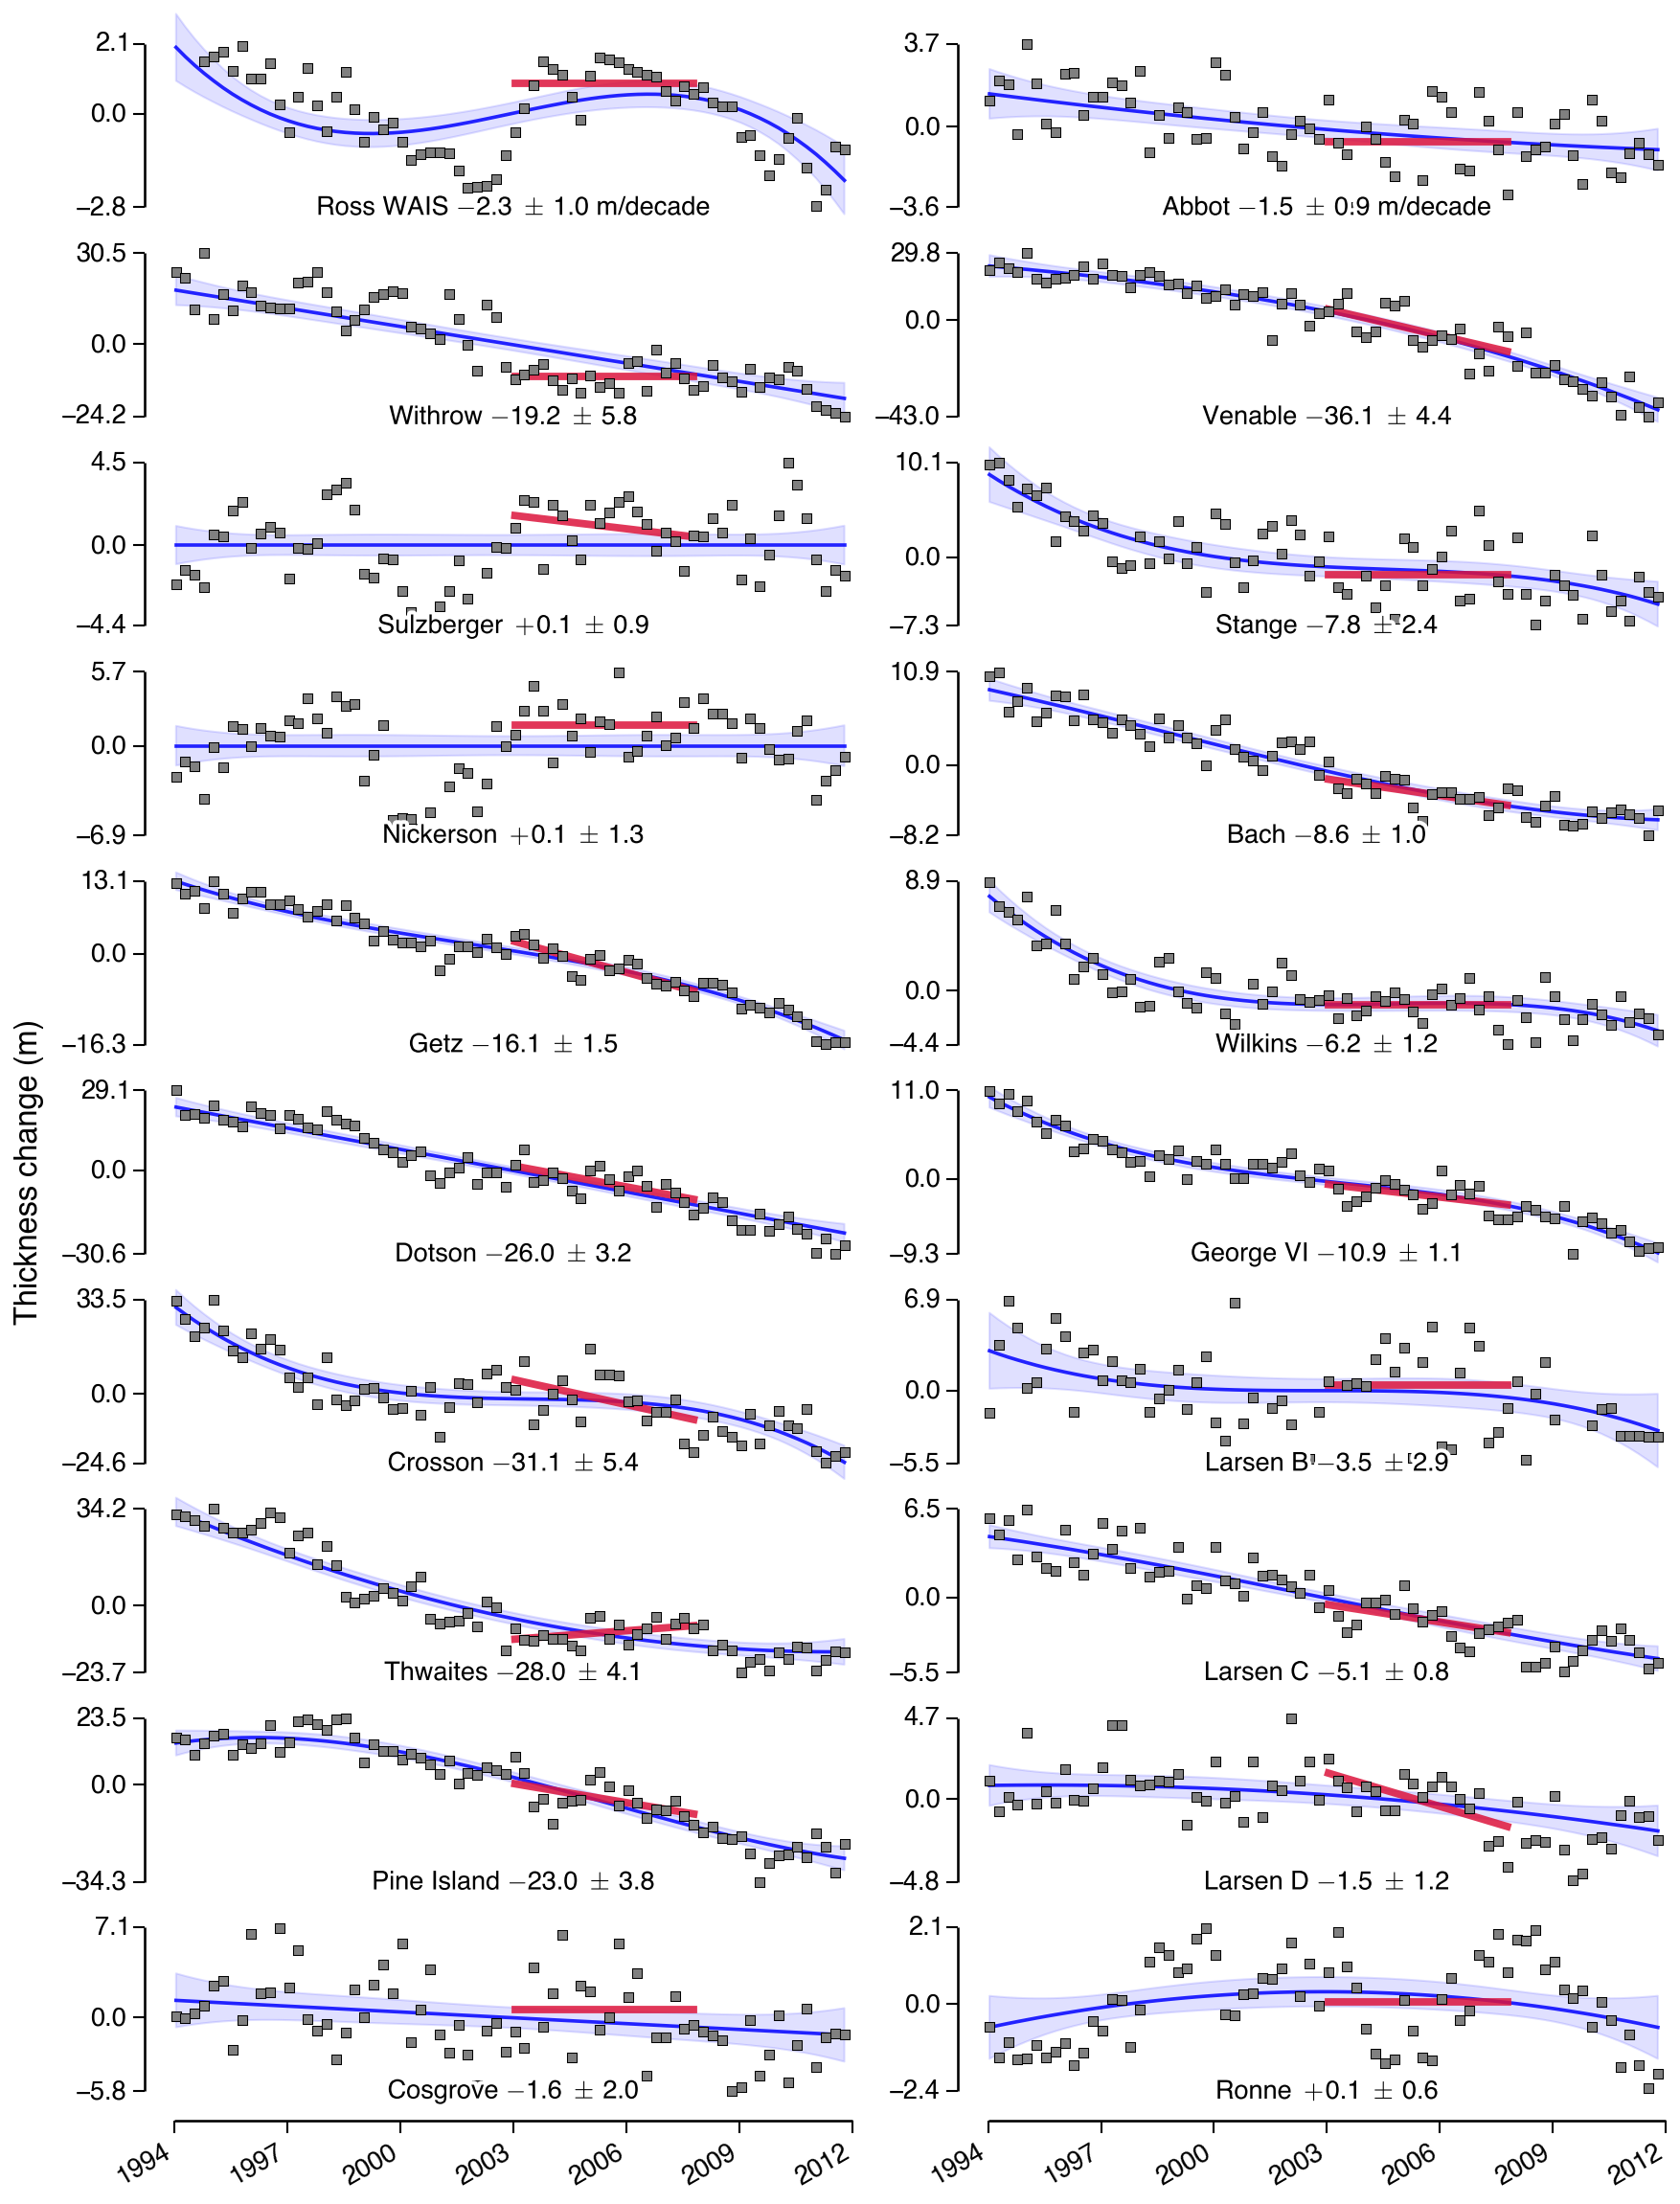
\includegraphics[width=.95\textwidth]{img/Sup1_ts_shelves_weis_review_v6.png}
  \caption[Time series of cumulative thickness change for West]{
  \ssp \footnotesize
Time series of cumulative thickness change for West Antarctic ice shelves relative to series means. Thickness change was averaged over the extent of each ice shelf (sampled area only) for the period 1994--2012. Clock-wise from Ross-WAIS to Ronne. Locations are shown in Fig.~\ref{fig:ice-shelf-change}. Black dots are 3-month-average thickness changes relative to series mean, blue curve is the 18-year polynomial trend with the 95\% confidence band, and red line shows the regression line to the segment of our dataset that overlaps with the period used for a prior ICESat-based analysis (2003--2008) \parencite{Pritchard2012}. Average rates (in m/decade) are derived from the end points of the polynomial models.
  }
  \label{fig:ts-ice-shelves-wais}
\end{figure}

\begin{figure}[!h]
  \centering
  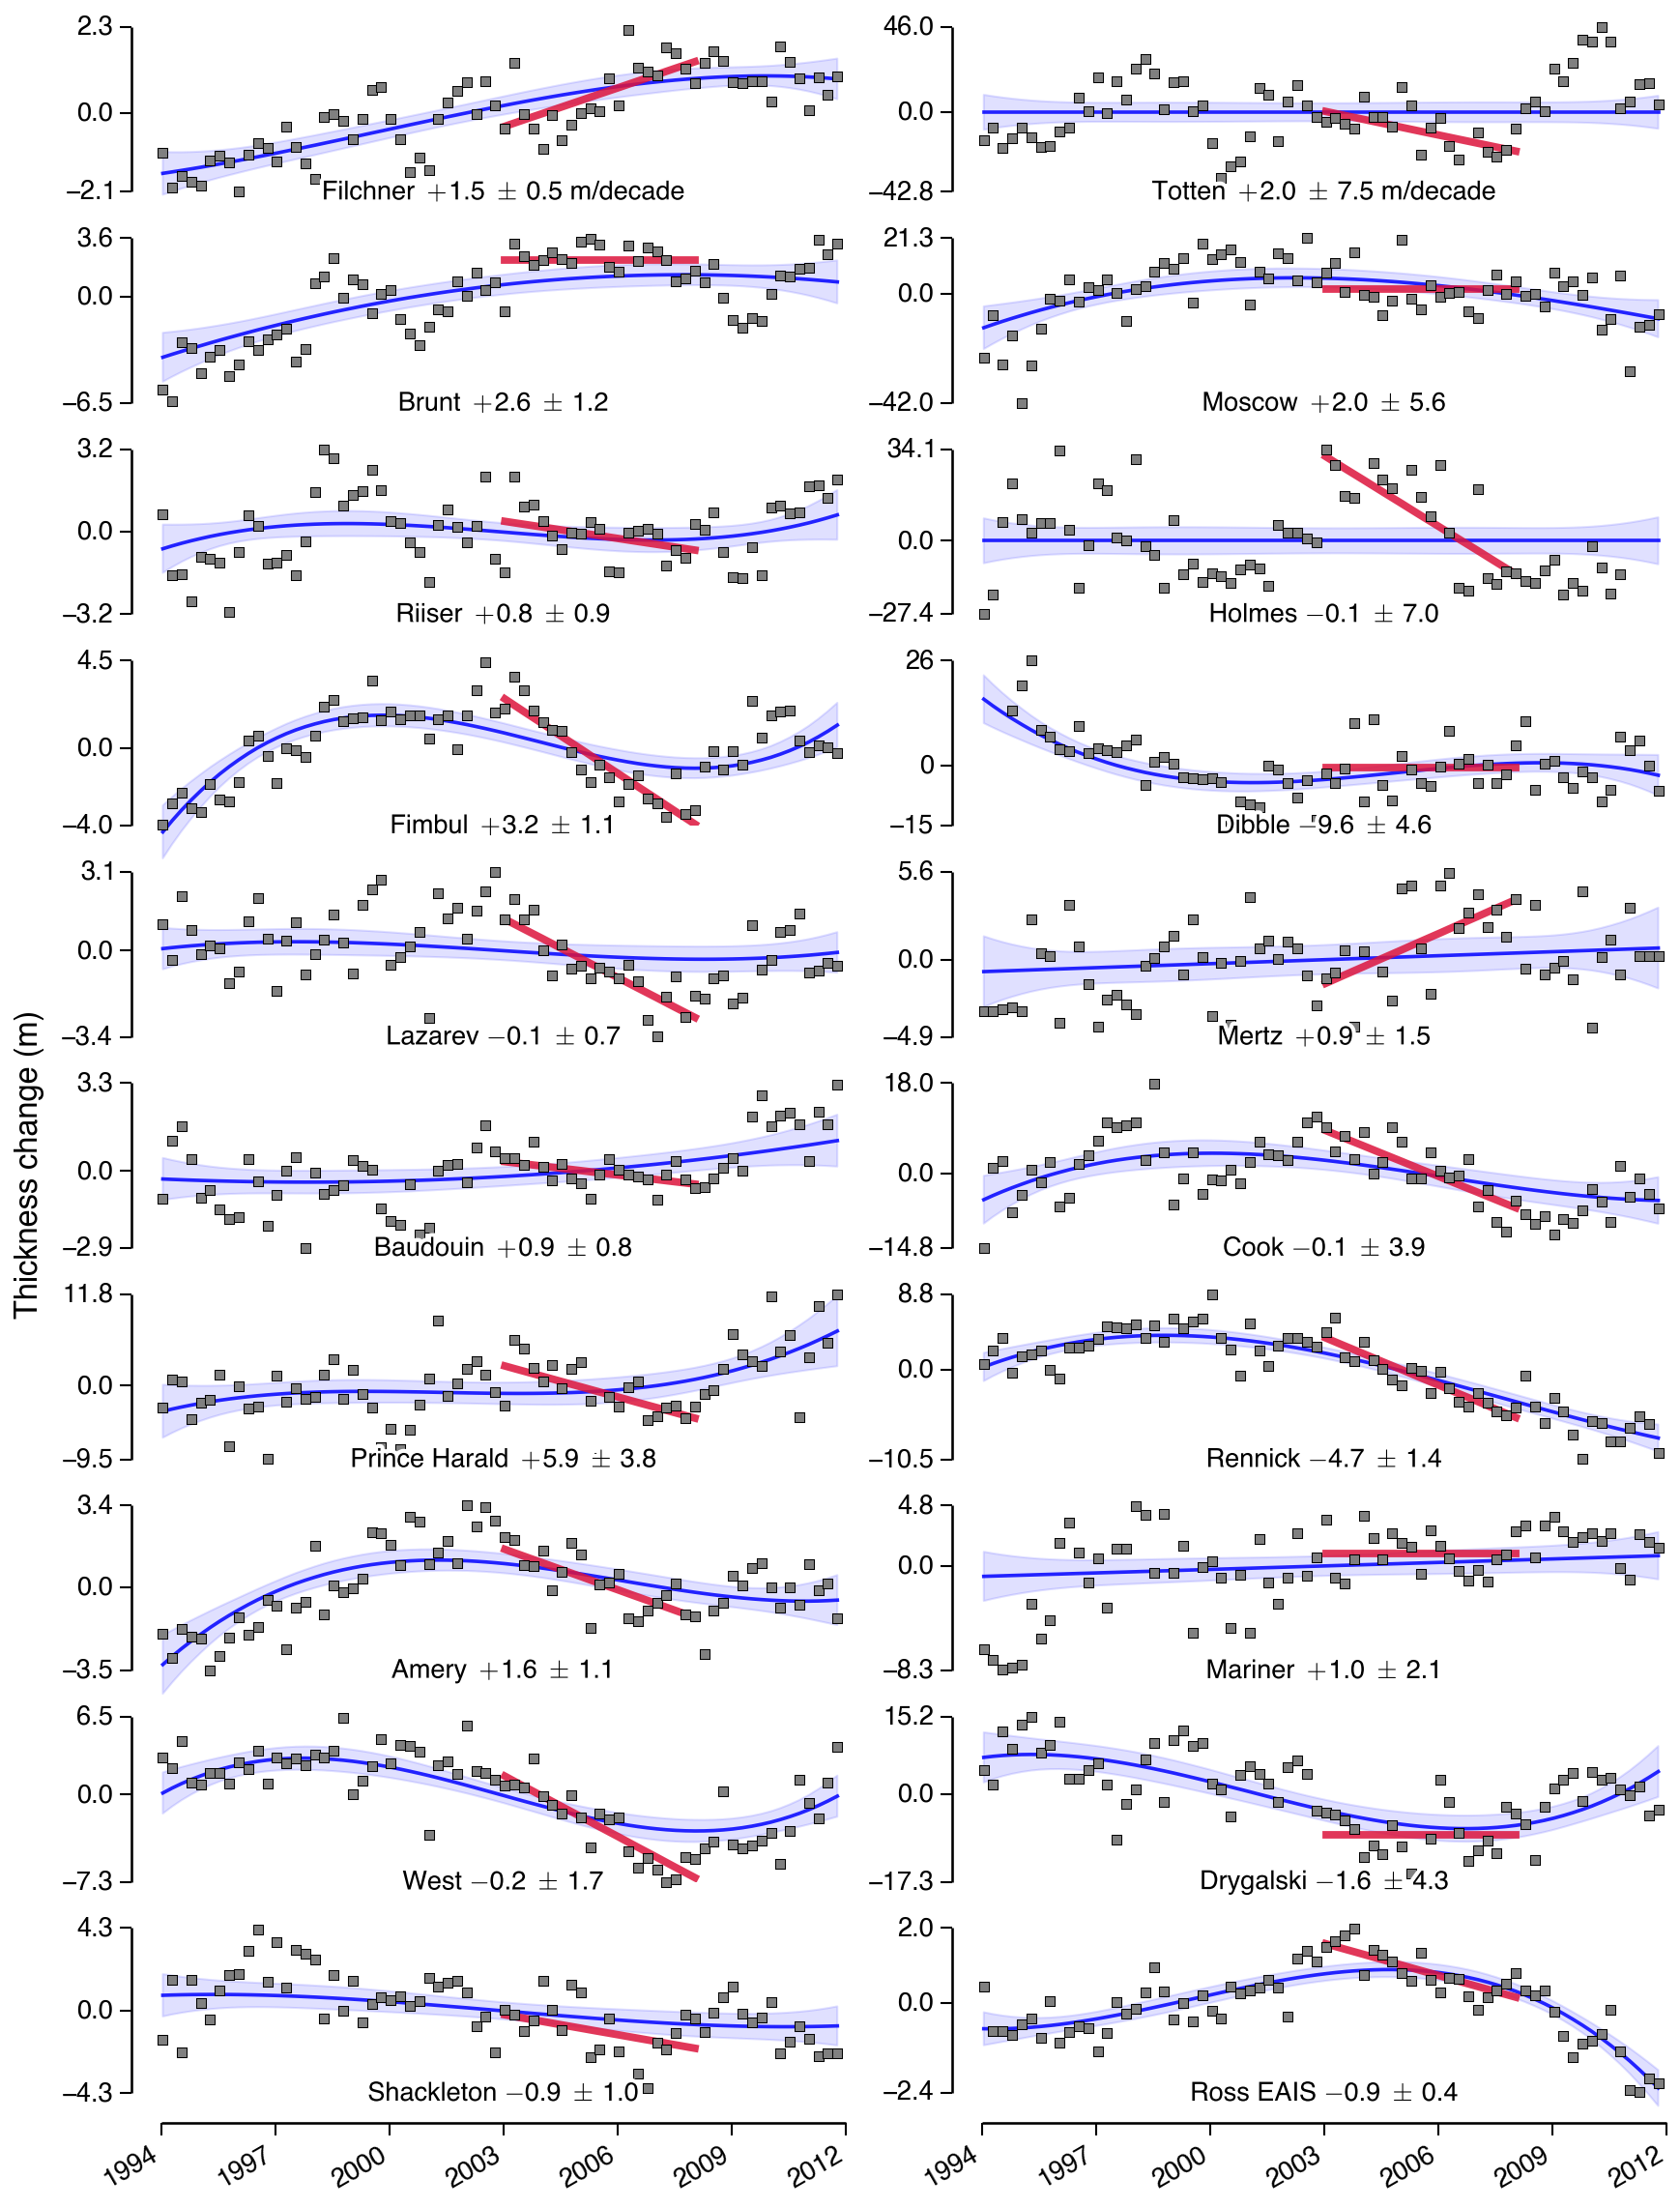
\includegraphics[width=.95\textwidth]{img/Sup1_ts_shelves_eais_review_v7.png}
  \caption[Time series of cumulative thickness change for East]{
  \ssp \footnotesize
Time series of cumulative thickness change for East Antarctic ice shelves relative to series mean. Thickness change was averaged over the extent of each ice shelf (sampled area only) for the period 1994--2012. Clock-wise from Filchner to Ross-EAIS. Locations are shown in Fig.~\ref{fig:ice-shelf-change}. Black dots are 3-month-average thickness changes relative to series mean, blue curve is the 18-year polynomial trend with the 95\% confidence band, and red line shows the regression line to the segment of our dataset that overlaps with the period used for a prior ICESat-based analysis (2003--2008) \parencite{Pritchard2012}. Average rates (in m/decade) are derived from the end points of the polynomial models.
}
  \label{fig:ts-ice-shelves-east}
\end{figure}


\begin{figure}[!h]
  \centering
  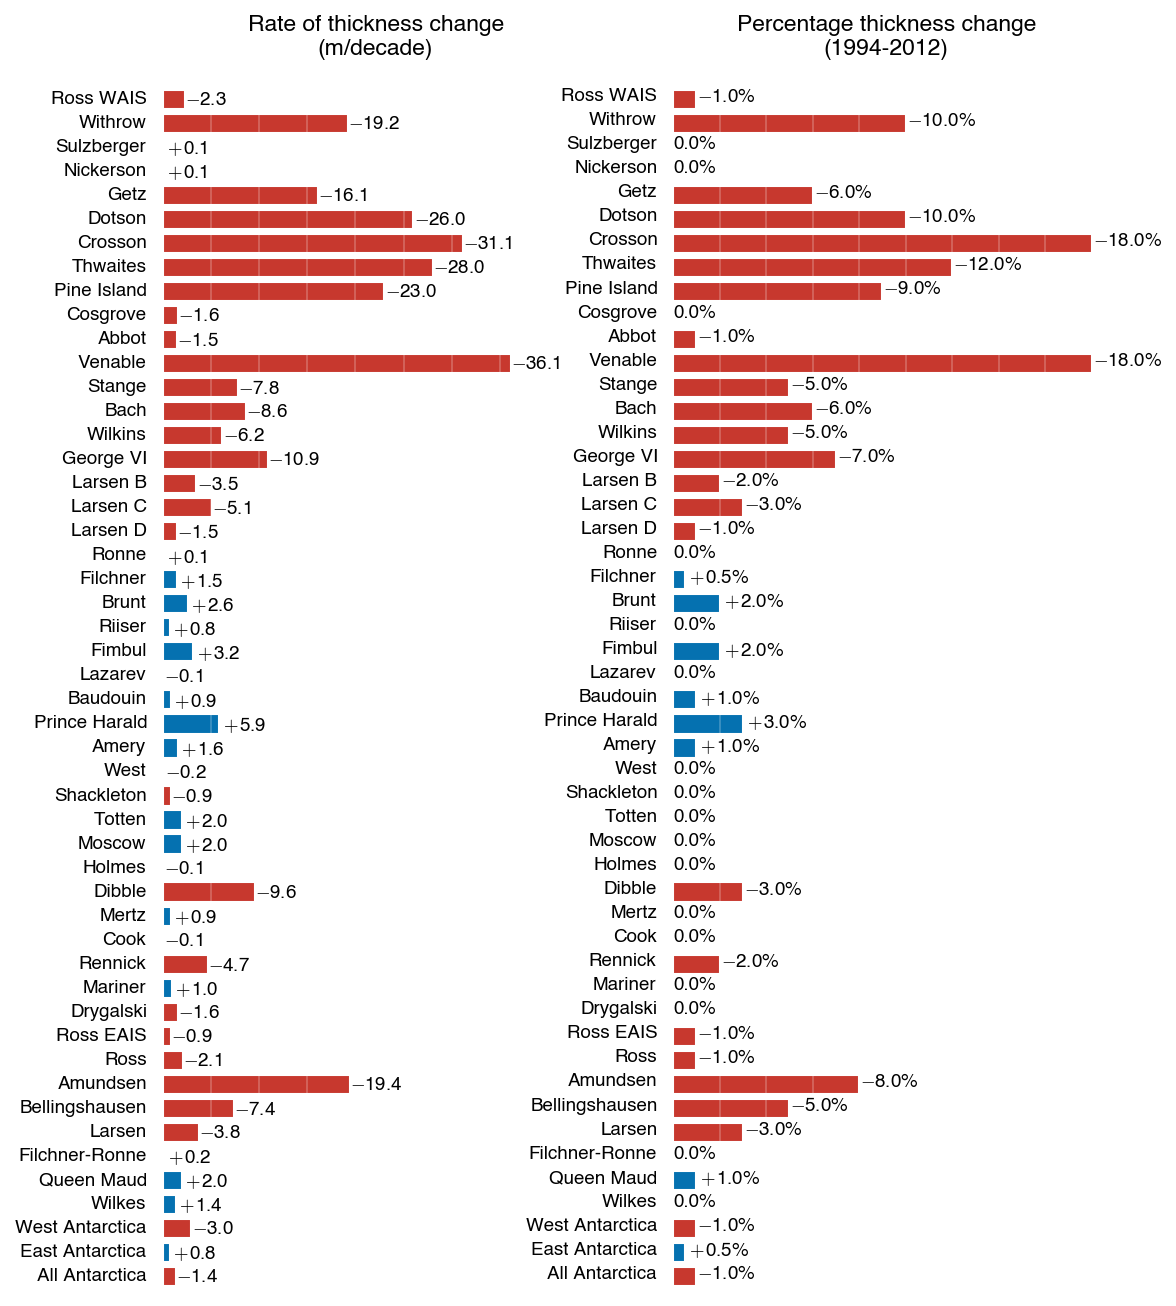
\includegraphics[width=\textwidth]{img/Sup2_barchart1_review_v7.png}
  \caption[Average rate and total thickness change for each Antarctic]{
  \ssp \footnotesize
  Average rate and total thickness change for each Antarctic ice shelf from 1994 to 2012. (left) Rate of thickness change (in m/decade) and (right) percentage thickness lost or gained in 18 years (values not significant at the 95\% confidence level were set to 0\%). Values are grouped as: West Antarctic ice shelves (top), East Antarctic ice shelves (middle) and regions (bottom). Red is thinning/loss and blue is thickening/gain. Locations are shown in Fig.~\ref{fig:ice-shelf-change}.
  }
  \label{c3f6}
\end{figure}


\begin{figure}[!h]
  \centering
  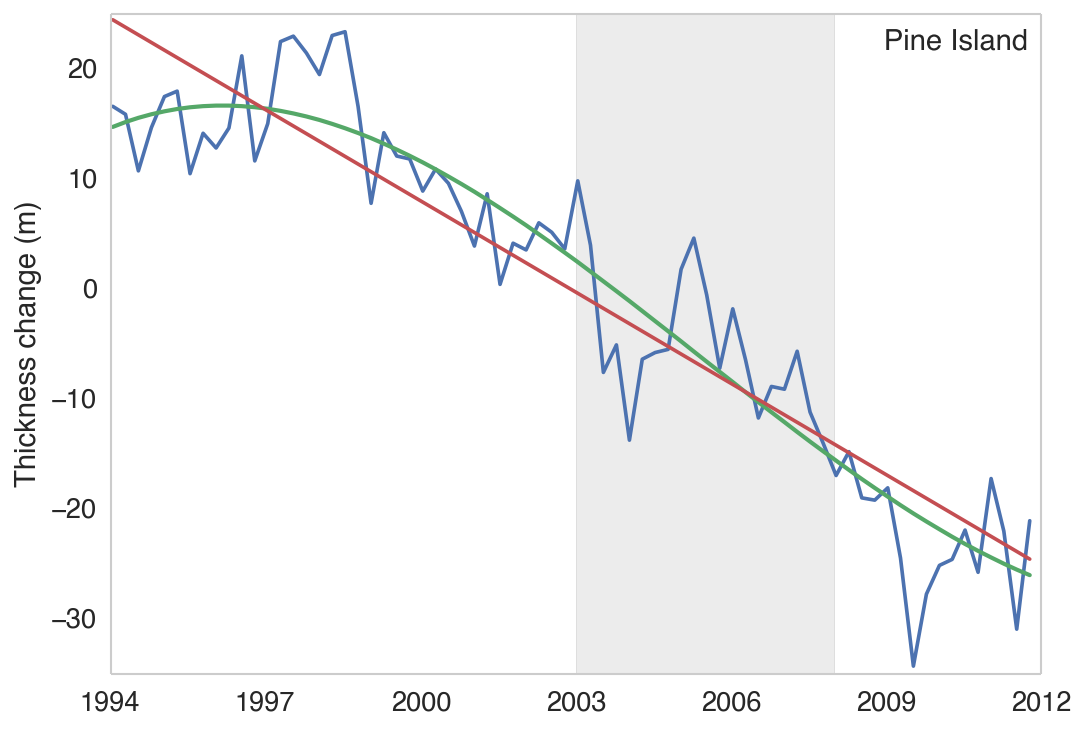
\includegraphics[width=.74\textwidth]{img/ts_pig_v2.png}\\
  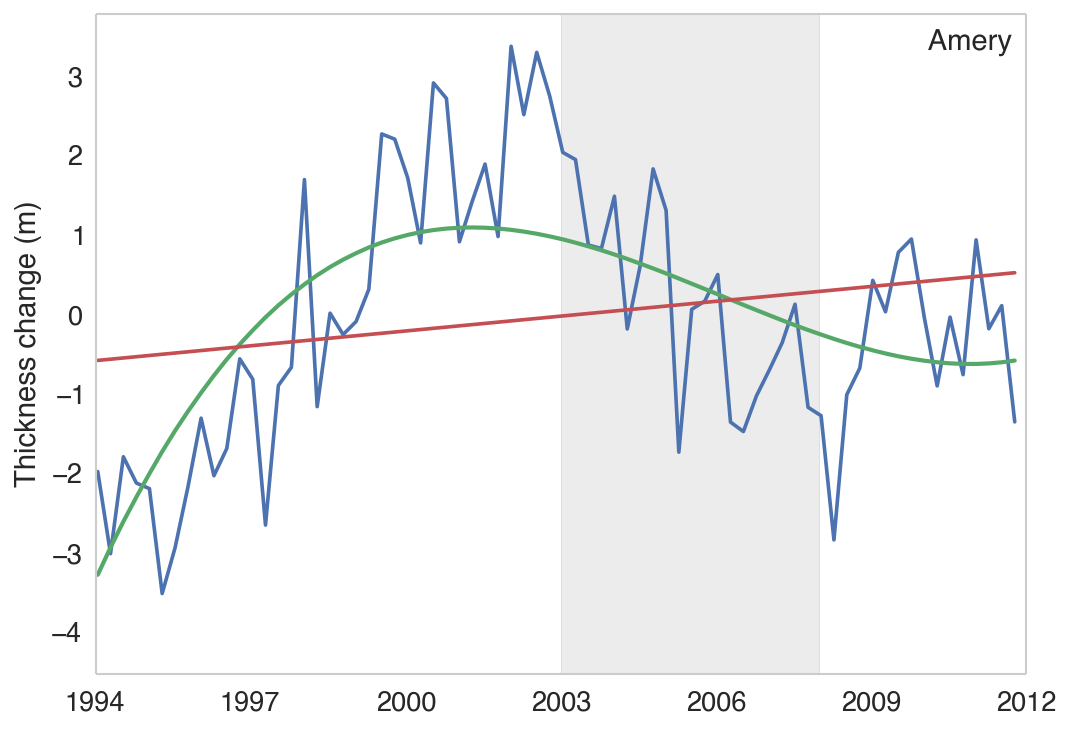
\includegraphics[width=.74\textwidth]{img/ts_amery_v2.png}
  \caption[Polynomial versus line fit to 18-year-long records]{
  \ssp \footnotesize
Polynomial versus line fit to 18-year-long records. Examples of discrepancies between polynomial regression (green) and straight-line fit (red) in representing long-term trends in thickness-change time series (blue). Two examples showing (top) Pine Island Ice Shelf and (bottom) Amery Ice Shelf, where the straight-line fit overestimates and underestimates, respectively, the trend. The shaded region (light gray) represents the time interval used in a previous ICESat-based study (2003--2008) \parencite{Pritchard2012}.
  }
  \label{c3f7}
\end{figure}


\begin{figure}[!h]
  \centering
  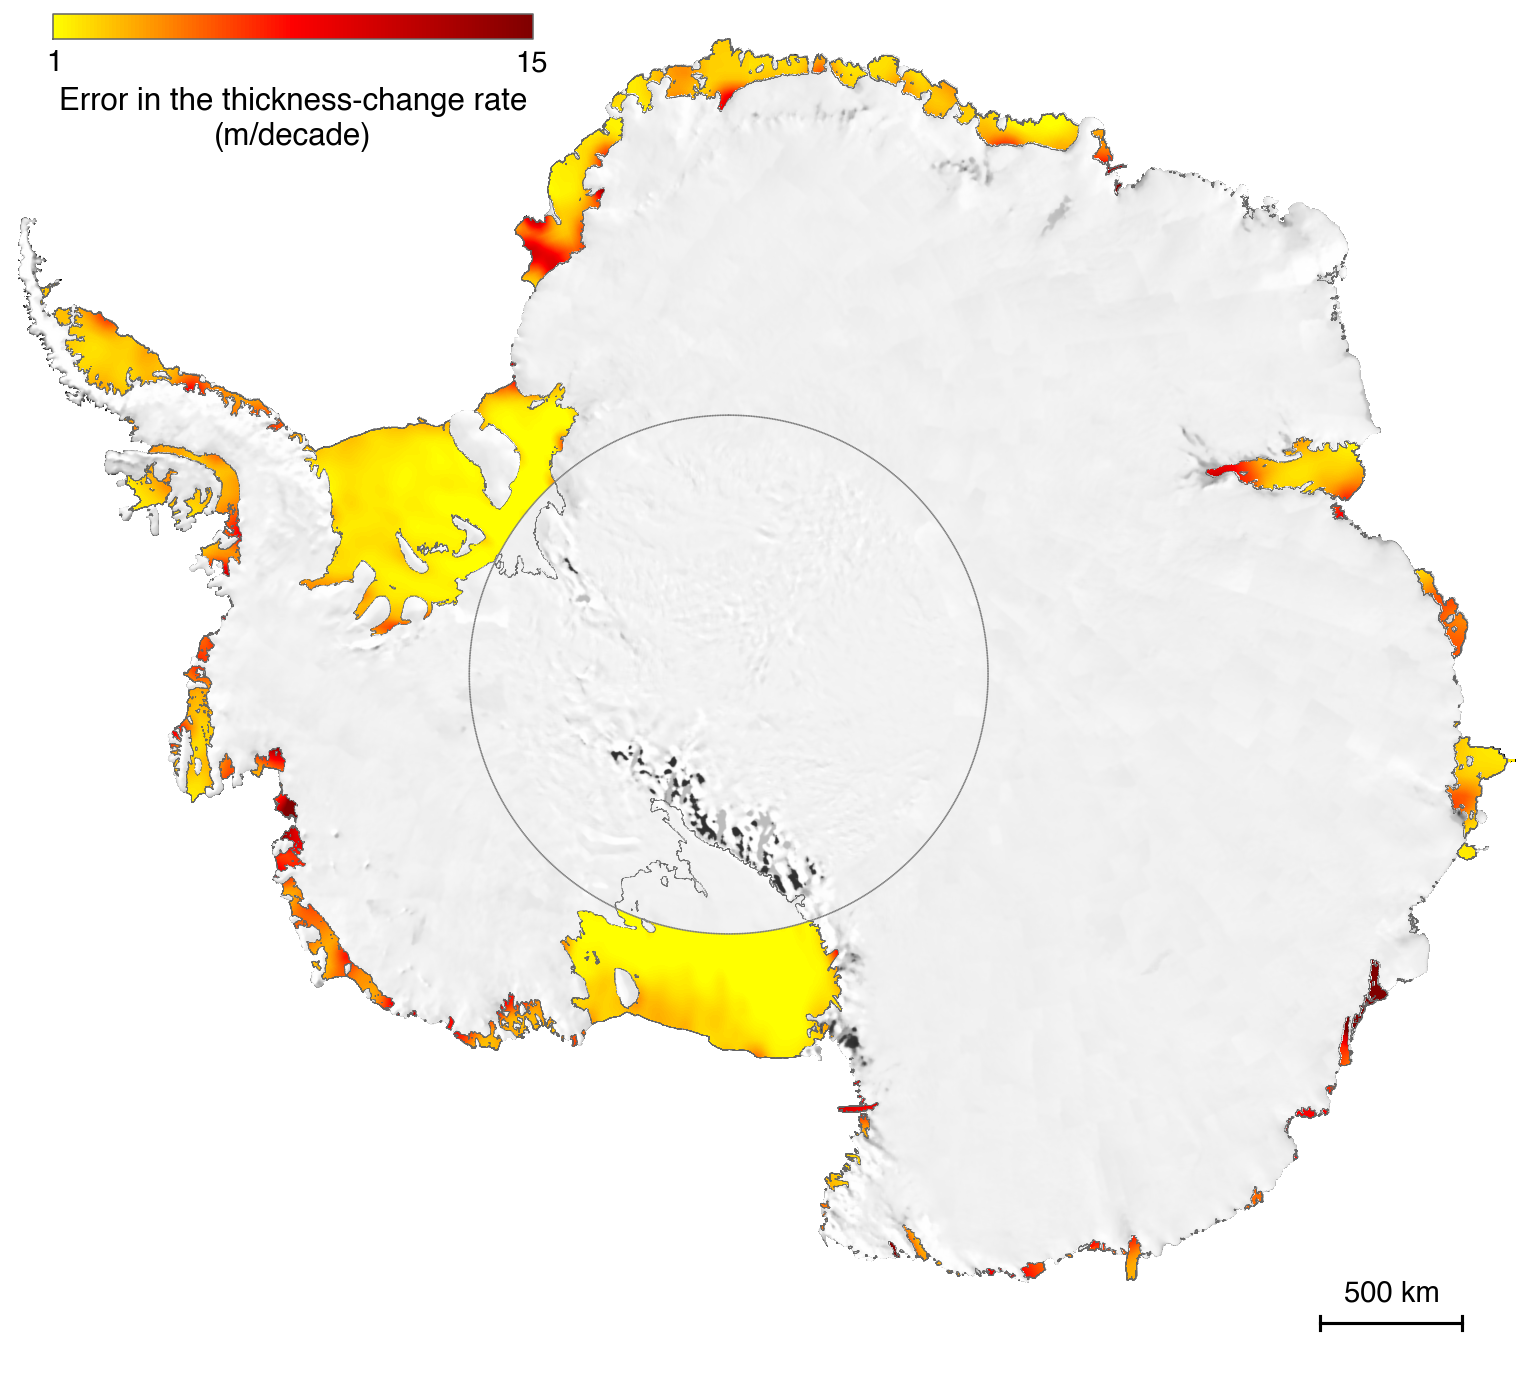
\includegraphics[width=\textwidth]{img/Sup4_error_review_v6.png}
  \caption[Error map for estimated rates of Antarctic ice-shelf]{
  \ssp \footnotesize
Error map for estimated rates of Antarctic ice-shelf thickness change. Map showing estimated uncertainties for individual (grid cell) decade-averaged rates of thickness change (map on Fig.~\ref{fig:ice-shelf-change}). Uncertainties are two standard errors (95\% confidence level) estimated using the bootstrap approach \parencite[see text;][]{Efron1993}.
  }
  \label{c3f8}
\end{figure}


\clearpage
\begin{footnotesize}
%\begin{longtable}{p{.13\textwidth}p{.15\textwidth}p{.15\textwidth}p{.15\textwidth}p{.14\textwidth}p{.11\textwidth}} 
\begin{longtable}{lrrrrr}
\caption[Average rates and total thickness change for Antarctic ice]{
  \ssp \footnotesize
Average rates and total thickness change for Antarctic ice shelves from 1994 to 2012. Table summarizing estimated area, decade-averaged ice-shelf-wide and local-minimum thickness-change rates, volume-change rate and percentage-thickness change during 1994--2012, for each Antarctic ice shelf and region. Uncertainties are stated at the 95\% confidence level. Total area refers to area under the satellite's coverage (latitudinal limit of 81.5$^\circ$S). Percentages have been rounded to the next integer or to $\pm$0.5 when below 1\% (only significant values have been considered). Note: Small differences are due to values being computed independently (subject to different constraints on the regression analysis from individual datasets), and use of round-off values. All estimates are consistent within the formal errors.
} \\
\hline
Ice shelf       & Area (Survey)    & Thickness rate  & Local minimum    & Volume rate   & \%--Change \\
                & (km$^2$)         & (m/decade)      & (m/decade)       & (km$^3$/year) & 1994--2012 \\
\hline
\endfirsthead   % this appears at the top one time only
\multicolumn{6}{l}%
{{\bfseries \tablename\ \thetable{}:} Average rates and total thickness change for Antarctic ice shelves (continued).} \\
\hline
Ice shelf       & Area (Survey)    & Thickness rate  & Local minimum    & Volume rate   & \%--Change \\
                & (km$^2$)         & (m/decade)      & (m/decade)       & (km$^3$/year) & 1994--2012 \\
\hline
\endhead        % this appears at the top of each chunk (page)
\hline
{\it continues...}
\endfoot        % this appears at the bottom of each chunk (page)
\hline
\endlastfoot    % this appears at the final bootom
%
Ross WAIS       & 215,000   (97\%) & $-2.3  \pm 1.0$ & $-35.0 \pm 10.0$ & $-48  \pm 22$ & $-1  $ \\
Withrow 	& 650       (82\%) & $-19.2 \pm 5.8$ & $-19.2 \pm 5.8 $ & $-2   \pm 1 $ & $-10 $ \\
Sulzberger 	& 12,200    (78\%) & $0.1   \pm 0.9$ & $-6.8  \pm 4.2 $ & $0    \pm 1 $ &  ---   \\
Nickerson 	& 6,600     (80\%) & $0.1   \pm 1.3$ & $-15.7 \pm 3.0 $ & $0    \pm 1 $ &  ---   \\
Getz 	        & 33,200    (85\%) & $-16.1 \pm 1.5$ & $-66.5 \pm 9.0 $ & $-54  \pm 5 $ & $-6  $ \\
Dotson  	& 5,400     (80\%) & $-26.0 \pm 3.2$ & $-64.5 \pm 7.9 $ & $-14  \pm 2 $ & $-10 $ \\
Crosson 	& 2,700     (78\%) & $-31.1 \pm 5.4$ & $-31.4 \pm 8.6 $ & $-8   \pm 2 $ & $-18 $ \\
Thwaites 	& 4,600     (75\%) & $-28.0 \pm 4.1$ & $-31.7 \pm 4.4 $ & $-13  \pm 2 $ & $-12 $ \\
Pine Island 	& 6,000     (60\%) & $-23.0 \pm 3.8$ & $-34.7 \pm 4.7 $ & $-14  \pm 2 $ & $-9  $ \\
Cosgrove 	& 3,000     (65\%) & $1.6   \pm 2.0$ & $-29.2 \pm 8.2 $ & $0    \pm 1 $ &  ---   \\
Abbot 	        & 30,100    (80\%) & $-1.5  \pm 0.9$ & $-19.2 \pm 4.4 $ & $-4   \pm 3 $ & $-1  $ \\
Venable 	& 3,100     (85\%) & $-36.1 \pm 4.4$ & $-64.4 \pm 4.9 $ & $-11  \pm 1 $ & $-18 $ \\
Stange 	        & 7,700     (80\%) & $-7.8  \pm 2.4$ & $-15.1 \pm 2.1 $ & $-6   \pm 2 $ & $-5  $ \\
Bach 	        & 4,600     (60\%) & $-8.6  \pm 1.0$ & $-12.9 \pm 1.3 $ & $-4   \pm 1 $ & $-6  $ \\
Wilkins 	& 13,500    (82\%) & $-6.2  \pm 1.2$ & $-19.9 \pm 2.0 $ & $-8   \pm 2 $ & $-5  $ \\
George VI 	& 23,200    (75\%) & $-10.9 \pm 1.1$ & $-31.3 \pm 6.7 $ & $-25  \pm 3 $ & $-7  $ \\
Larsen B 	& 2,500     (50\%) & $-3.5  \pm 2.9$ & $-5.5  \pm 2.9 $ & $-1   \pm 1 $ & $-2  $ \\
Larsen C 	& 46,500    (96\%) & $-5.1  \pm 0.8$ & $-16.6 \pm 8.1 $ & $-24  \pm 4 $ & $-3  $ \\
Larsen D 	& 25,000    (70\%) & $-1.5  \pm 1.2$ & $-22.5 \pm 2.8 $ & $-4   \pm 3 $ & $-1  $ \\
Ronne 	        & 318,000   (98\%) & $0.1   \pm 0.6$ & $-10.0 \pm 3.5 $ & $2    \pm 19$ &  ---   \\
Filchner 	& 91,000    (95\%) & $1.5   \pm 0.5$ & $-12.7 \pm 1.7 $ & $13   \pm 4 $ & $0.5 $ \\
Brunt 	        & 36,000    (78\%) & $2.6   \pm 1.2$ & $-24.5 \pm 7.8 $ & $9    \pm 4 $ & $2   $ \\
Riiser  	& 43,000    (90\%) & $0.8   \pm 0.9$ & $-3.7  \pm 1.5 $ & $3    \pm 4 $ &  ---   \\
Fimbul  	& 40,500    (78\%) & $3.2   \pm 1.1$ & $-7.7  \pm 2.5 $ & $13   \pm 5 $ & $2   $ \\
Lazarev 	& 8,500     (75\%) & $-0.1  \pm 0.7$ & $-1.6  \pm 1.5 $ & $0    \pm 1 $ &  ---   \\
Baudouin 	& 33,000    (80\%) & $0.9   \pm 0.8$ & $-7.0  \pm 8.5 $ & $3    \pm 2 $ & $1   $ \\
Prince Harald 	& 5,000     (50\%) & $5.9   \pm 3.8$ & $-0.3  \pm 2.1 $ & $3    \pm 2 $ & $3   $ \\
Amery 	        & 60,000    (88\%) & $1.6   \pm 1.1$ & $-18.3 \pm 9.2 $ & $9    \pm 6 $ & $1   $ \\
West 	        & 15,500    (50\%) & $-0.2  \pm 1.7$ & $-21.3 \pm 5.7 $ & $0    \pm 3 $ &  ---   \\
Shackleton 	& 31,000    (48\%) & $-0.9  \pm 1.0$ & $-9.3  \pm 9.2 $ & $-3   \pm 3 $ &  ---   \\
Totten  	& 6,000     (50\%) & $2.0   \pm 7.5$ & $2.0   \pm 7.5 $ & $1    \pm 5 $ &  ---   \\
Moscow  	& 5,600     (50\%) & $2.0   \pm 5.6$ & $-5.7  \pm 4.2 $ & $1    \pm 3 $ &  ---   \\
Holmes  	& 2,000     (40\%) & $-0.1  \pm 7.0$ & $-0.4  \pm 7.4 $ & $0    \pm 1 $ &  ---   \\
Dibble  	& 1,500     (60\%) & $-9.6  \pm 4.6$ & $-9.6  \pm 4.6 $ & $-2   \pm 1 $ & $-3  $ \\
Mertz 	        & 2,800     (55\%) & $0.9   \pm 1.5$ & $0.9   \pm 1.5 $ & $1    \pm 2 $ &  ---   \\
Cook 	        & 3,200     (35\%) & $-0.1  \pm 3.9$ & $-22.9 \pm 4.0 $ & $0    \pm 1 $ &  ---   \\
Rennick 	& 3,200     (80\%) & $-4.7  \pm 1.4$ & $-17.1 \pm 2.2 $ & $-2   \pm 1 $ & $-2  $ \\
Mariner 	& 2,600     (55\%) & $1.0   \pm 2.1$ & $1.0   \pm 2.1 $ & $0    \pm 1 $ &  ---   \\
Drygalski 	& 2,500     (50\%) & $-1.6  \pm 4.3$ & $-14.4 \pm 11.2$ & $0    \pm 1 $ &  ---   \\
Ross EAIS 	& 145,000   (98\%) & $-0.9  \pm 0.4$ & $-32.9 \pm 8.3 $ & $-13  \pm 6 $ & $-1  $ \\
Ross	        & 360,000   (98\%) & $-2.1  \pm 0.5$ & $-35.0 \pm 10.0$ & $-75  \pm 19$ & $-1  $ \\
Amundsen 	& 56,000    (80\%) & $-19.4 \pm 1.9$ & $-66.5 \pm 9.0 $ & $-109 \pm 11$ & $-8  $ \\
Bellingshausen  & 86,000    (78\%) & $-7.4  \pm 0.9$ & $-64.4 \pm 4.9 $ & $-64  \pm 8 $ & $-5  $ \\
Larsen  	& 75,000    (80\%) & $-3.8  \pm 1.1$ & $-22.5 \pm 2.8 $ & $-28  \pm 8 $ & $-3  $ \\
Filchner-Ronne  & 410,000   (97\%) & $0.2   \pm 0.5$ & $-12.7 \pm 1.7 $ & $5    \pm 22$ &  ---   \\
Queen Maud 	& 224,000   (78\%) & $2.0   \pm 0.8$ & $-24.5 \pm 7.8 $ & $44   \pm 18$ & $1   $ \\
Wilkes  	& 87,000    (55\%) & $1.4   \pm 1.5$ & $-22.9 \pm 4.0 $ & $12   \pm 13$ &  ---   \\
West Antarctica & 650,000   (90\%) & $-3.0  \pm 0.5$ & $-66.5 \pm 9.0 $ & $-191 \pm 32$ & $-1  $ \\
East Antarctica & 600,000   (82\%) & $0.8   \pm 0.5$ & $-32.9 \pm 8.3 $ & $45   \pm 29$ & $0.5 $ \\
All Antarctica  & 1,250,000 (86\%) & $-1.4  \pm 0.4$ & $-66.5 \pm 9.0 $ & $-166 \pm 48$ & $-1  $ \\[-.55cm]
%
\label{tab:estimates}
\end{longtable}
\end{footnotesize}


\clearpage
\begin{footnotesize}
\begin{longtable}{lrrrr} 
\caption[Comparison of our estimated thickness-change rates]{
  \ssp \footnotesize
Comparison of our estimated thickness-change rates (m/year) with previous studies. Table comparing our estimates \parencite{Paolo2015} with \textcite{Pritchard2012}, \textcite{Shepherd2010} and \textcite{Shepherd2004}. Missing values correspond to either different ice-shelf boundary definition or ice shelf not reported. When required, we converted all the estimates to thickness change (in m/year) and rounded values to facilitate the comparison. Values not significantly different from zero were set to 0.0. See text for explanation on potential differences.
}\\

\hline
Ice shelf       & Paolo {\it et al.}\footnotemark[1] & Pritchard {\it et al.}\footnotemark[2]   & Shepherd {\it et al.}\footnotemark[3] & Shepherd {\it et al.}\footnotemark[4] \\
                & 18 years               & 5 years                      & 9 years                   & 14 years                  \\
                & (1994--2012)           & (2003--2008)                 & (1992--2001)              & (1994--2008)              \\
\hline
\endfirsthead   % this appears at the top one time only
\multicolumn{5}{l}%
{{\bfseries \tablename\ \thetable{}:} Comparison of our estimated thickness-change rates (continued).} \\
\hline
Ice shelf       & Paolo {\it et al.}\footnotemark[1] & Pritchard {\it et al.}\footnotemark[2]   & Shepherd {\it et al.}\footnotemark[3] & Shepherd {\it et al.}\footnotemark[4] \\
                & 18 years               & 5 years                      & 9 years                   & 14 years                  \\
                & (1994--2012)           & (2003--2008)                 & (1992--2001)              & (1994--2008)              \\
\hline
\endhead        % this appears at the top of each chunk (page)
\hline
{\it continues...}
\endfoot        % this appears at the bottom of each chunk (page)
\hline
\endlastfoot    % this appears at the final bootom
%
Sulzberger     & $0.0 $ & $0.3 $ &  ---   &  ---    \\
Nickerson      & $0.0 $ & $0.0 $ &  ---   &  ---    \\	
Getz	       & $-1.6$ & $-1.7$ & $-1.6$ & $-1.8 $ \\
Dotson	       & $-2.6$ & $-5.2$ & $-3.3$ &  ---    \\
Crosson	       & $-3.1$ & $-3.3$ & $-4.5$ &  ---    \\
Thwaites       & $-2.8$ & $-5.6$ & $-5.5$ & $-8.3 $ \\
Pine Island    & $-2.3$ & $-4.9$ & $-3.9$ & $-6.0 $ \\
Cosgrove       & $-0.2$ & $-0.6$ & $-0.7$ &  ---    \\
Abbot	       & $-0.2$ & $0.4 $ & $-0.6$ &  ---    \\
Venable	       & $-3.6$ & $-2.5$ &  ---   & $-16.0$ \\
Stange	       & $-0.8$ & $-0.6$ &  ---   &  ---    \\
Bach	       & $-0.9$ & $-0.7$ &  ---   & $8.8  $ \\
Wilkins	       & $-0.6$ & $-0.6$ &  ---   &  ---    \\
George VI      & $-1.1$ & $-0.9$ &  ---   & $-0.8 $ \\
Larsen B       & $-0.4$ & $-2.3$ &  ---   &  ---    \\
Larsen C       & $-0.5$ & $-0.9$ &  ---   & $-0.8 $ \\
Larsen D       & $-0.2$ & $0.4 $ &  ---   &  ---    \\
Brunt	       & $0.3 $ & $0.3 $ &  ---   & $0.6  $ \\
Riiser	       & $0.1 $ & $0.3 $ &  ---   &  ---    \\
Fimbul	       & $0.3 $ & $0.0 $ &  ---   & $-0.5 $ \\
Lazarev	       & $0.0 $ & $-0.6$ &  ---   &  ---    \\
Amery	       & $0.2 $ & $-0.6$ &  ---   & $0.9  $ \\
West	       & $0.0 $ & $-1.1$ &  ---   &  ---    \\
Shackleton     & $0.0 $ & $-1.1$ &  ---   &  ---    \\
Totten	       & $0.0 $ & $-3.8$ &  ---   &  ---    \\
Moscow	       & $0.0 $ & $-1.0$ &  ---   & $5.4  $ \\
Holmes	       & $0.0 $ & $-2.8$ &  ---   &  ---    \\
Dibble	       & $-1.0$ & $-2.2$ &  ---   &  ---    \\
Mertz	       & $0.0 $ & $0.3 $ &  ---   &  ---    \\
Cook	       & $0.0 $ & $1.1 $ &  ---   &  ---    \\
Rennick	       & $-0.5$ & $-1.2$ &  ---   &  ---    \\
Mariner	       & $0.0 $ & $0.2 $ &  ---   &  ---    \\
Drygalski      & $0.0 $ & $-0.3$ &  ---   &  ---    \\
Ross	       & $-0.2$ & $0.1 $ &  ---   & $0.2 $  \\
Filchner-Ronne & $0.0 $ & $0.2 $ &  ---   & $0.5 $  \\[-.55cm]
%
\footnotetext[1]{\textcite{Paolo2015}, Radar altimetry.}
\footnotetext[2]{\textcite{Pritchard2012}, Laser altimetry.}
\footnotetext[3]{\textcite{Shepherd2010}, Radar altimetry.}
\footnotetext[4]{\textcite{Shepherd2004}, Radar altimetry.}
\label{tab:comparison}
\end{longtable}
\end{footnotesize}


\clearpage
\section*{Acknowledgements}

This work was funded by NASA [awards NNX12AN50H 002
(93735A), NNX10A-G19G, and NNX13AP60G]. This is ESR
contribution 154. We thank J. Zwally's Ice Altimetry group
at the NASA Goddard Space Flight Center for distributing their
RA data sets for all satellite radar altimeter missions
(\url{http://icesat4.gsfc.nasa.gov}). We thank C. Davis and D. Wingham for
RA-processing advice. We thank A. Shepherd and anonymous
reviewers for their comments on the manuscript.


{\sl Chapter 3}, in full, is a reprint of the material as it appears in {\it Science}
2015. Paolo, Fernando S.; Fricker, Helen A.; Padman, Laurie. The dissertation
author was the primary investigator and author of this paper.

\printbibliography[segment=3,heading=subbibliography]

%%
% Chapter 2 - Methodology 
% -----------------------
% Jun 1, 2015
%

\chapter{Just a Test}
This is only a test.


\section{A section}
Lorem ipsum dolor sit amet, consectetuer adipiscing elit. Nulla odio
sem, bibendum ut, aliquam ac, facilisis id, tellus. Nam posuere pede
sit amet ipsum. Etiam dolor. In sodales eros quis pede.  Quisque sed
nulla et ligula vulputate lacinia. In venenatis, ligula id semper
feugiat, ligula odio adipiscing libero, eget mollis nunc erat id orci.
Nullam ante dolor, rutrum eget, vestibulum euismod, pulvinar at, nibh.
In sapien. Quisque ut arcu. Suspendisse potenti. Cras consequat cursus
nulla.


\subsection{More Stuff}
Blah

\begin{figure}[h] 
  \centering
  *
  \caption{A figure of Vonnegut.\index{Vonnegut}} 
\end{figure}



\appendix

%\printbibliography[segment=4,heading=subbibliography]

%
% Of course, if you prefer, you can just start with
%   \chapter{My First Chapter Name}
% and start typing away.  
%\chapter{Just a Test}
%This is only a test.
%\section{A section}
%Lorem ipsum dolor sit amet, consectetuer adipiscing elit. Nulla odio
%sem, bibendum ut, aliquam ac, facilisis id, tellus. Nam posuere pede
%sit amet ipsum. Etiam dolor. In sodales eros quis pede.  Quisque sed
%nulla et ligula vulputate lacinia. In venenatis, ligula id semper
%feugiat, ligula odio adipiscing libero, eget mollis nunc erat id orci.
%Nullam ante dolor, rutrum eget, vestibulum euismod, pulvinar at, nibh.
%In sapien. Quisque ut arcu. Suspendisse potenti. Cras consequat cursus
%nulla.
%\subsection{More Stuff}
%Blah
%
%\begin{figure}[h] 
%  \centering
%  *
%  \caption{A figure of Vonnegut.\index{Vonnegut}} 
%\end{figure}
%
%
%
%\appendix
%\chapter{Final notes}
%  Remove me in case of abdominal pain.





%% END MATTER
% \printindex %% Uncomment to display the index
% \nocite{Shepherd2010}  %% Put any references that you want to include in the bib 
%               but haven't cited in the braces.
% \bibliographystyle{alpha}  %% This is just my personal favorite style. 
%                              There are many others.
% \bibliography{myrefs}  %% This looks for the bibliography in myrefs.bib 
%                          which should be formatted as a bibtex file.
\end{document}

